%%%%%%%%%%%%%%%%%%%%%%%%%%%%%%%%%%%%%%%%%%%%%%%%%%%%%%%%%%%%%%%%%%%%%%%%%%%%%%%
% Author:  Pablo Alvarado
%
% Escuela de Ingeniería Electrónica
% Instituto Tecnológico de Costa Rica
%
% Tesis de Licenciatura
% 
% Phone:   +506 550 2106
% Fax:     +506 591 6629
% email:   palvarado@ietec.org
%
% $Id: main.tex 1513 2010-08-15 01:25:24Z palvarado $
%
%%%%%%%%%%%%%%%%%%%%%%%%%%%%%%%%%%%%%%%%%%%%%%%%%%%%%%%%%%%%%%%%%%%%%%%%%%%%%%%

% \documentclass is book
\documentclass[12pt,twoside,letterpaper]{book}

\usepackage[utf8]{inputenc}
\usepackage{ifthen}                     % provide if-then-else operators

% --------------------------------------------------------------------------
% Global variables required in document formatting
% --------------------------------------------------------------------------
%
% BOOK MODE
%
\newboolean{bookmode}                  % boolean used to control book format
% Ensure that only one of the next two lines is active:
\setboolean{bookmode}{true}           % turn book mode on
%\setboolean{bookmode}{false}           % turn book mode off

%
% DRAFT MODE
%
\newboolean{draftmode}                  % boolean used to control draft-mode
% Ensure that only one of the next two lines is active:
\setboolean{draftmode}{true}            % turn draft mode on
%\setboolean{draftmode}{false}           % turn draft mode off
% --------------------------------------------------------------------------
%
% GENERAL AUTHOR, TITLE AND KEYWORDS
%
% Nombre del Estudiante
\newcommand{\scriptAuthor}{Manuel Zumbado Corrales}

% Título de la tesis
\newcommand{\scriptTitle}{Implementación paralela del filtro DNLM-IIFFT en sistemas multi-nodo optimizado para la arquitectura Intel Xeon Phi Knights Landing} 

% Keywords
\newcommand{\scriptKeywords}{palabras, clave, ...}

% Descripción de la editorial
\newcommand{\boxeditorial}{%
}

% Para el PDF (cambiar si se desea otras cosas a lo indicado arriba
\newcommand{\pdfAuthor}{\scriptAuthor}
\newcommand{\pdfTitle}{\scriptTitle} 
\newcommand{\pdfKeywords}{\scriptKeywords}

% --------------------------------------------------------------------------

% include all packages and define all required general macros
%%%%%%%%%%%%%%%%%%%%%%%%%%%%%%%%%%%%%%%%%%%%%%%%%%%%%%%%%%%%%%%%%%%%%%%%%%%%%%%
% Author:  Pablo Alvarado
%
% Escuela de Electrónica
% Instituto Tecnológico de Costa Rica
%
% Phone:   +506 550 2106
% Fax:     +506 591 6629
% email:   palvarado@ietec.org
%
% $Id: macros.tex 1497 2010-08-09 17:04:26Z palvarado $
%
%%%%%%%%%%%%%%%%%%%%%%%%%%%%%%%%%%%%%%%%%%%%%%%%%%%%%%%%%%%%%%%%%%%%%%%%%%%%%%%

% Configuration of the exercises package, which is used to collect all
% problems and answers in the document.
\usepackage[exercisedelayed,answerdelayed,lastexercise]{exercise}
\renewcounter{Exercise}[chapter]
\renewcommand{\ExerciseName}{Problema}
\renewcommand{\theExercise}{\thechapter.\arabic{Exercise}}
\newcommand{\ExerciseLabel}{Exercise.\theExercise}
\renewcommand{\ExerciseHeader}%
{\textbf{\ExerciseName\ \theExercise.\ \ExerciseHeaderTitle\ }}
\renewcommand{\AnswerHeader}%
{\textbf{\ExerciseName\ \theExercise.\ }}


\usepackage{ifpdf}

% Command to change between draft or release mode:
\newcommand{\ifdraft}[2]{\ifthenelse{\boolean{draftmode}}{#1}{#2}}
% Command to change between draft or release mode:
\newcommand{\ifbook}[2]{\ifthenelse{\boolean{bookmode}}{#1}{#2}}

% include all required packages here
\usepackage[spanish]{babel}     % supports english, but default is 
                                        % spanish...
\newcommand*{\SelectSpanish}{%          % well, the last line indeed selects
  \hyphenrules{spanish}%                % english over spanish, but with this
  \languageshorthands{spanish}%         % command we turn it around.
  \captionsspanish                      % The reason: hyperref has some
  \datespanish                          % problems with the spanish babel,
}                                       % so we use some trick here so that 
%\AtBeginDocument{\SelectSpanish}       % it thinks it is english.

\usepackage{makeidx}                    % to create index file

\ifdraft{%
  %\usepackage[refpage]{nomencl}        % Use to easily administrate the list
 \usepackage{nomencl}                   % of symbols
}{%
 \usepackage{nomencl}
}
%\usepackage{times}                     % replace latex pk fonts with ps type I
                                        % don't forget to use dvips -D600 -Pcmz
                                        % to ensure Type I fonts!
\usepackage{amsmath}
\usepackage{amssymb,amstext}            % AMS-math and symbols package
\usepackage{mathrsfs}                   % Calygraphic fonts for transforms
\usepackage{array}                      % extensions to tabular environment
\usepackage{longtable}                  % supports extraordinary long tables
\usepackage{tabularx}                   % supports tables with fixed width
\usepackage{afterpage}                  % put something only after the page
\usepackage{multirow}                   % supports multiple row grouping in 
                                        % tables
\usepackage{multicol}                   % multiple columns environments
\usepackage{paralist}                   % a few enumeration settings

\usepackage[hang,%
            small,%
            bf]{caption}                % nicer figure captions
%\usepackage{sty/ftcap}                 % switch \abovecaptionskip and
%                                       % \belowcaptionskip for tables, in 
%                                       % order to avoid the caption to be
%                                       % too near to the table itself
% locally added packages
\usepackage{float}                      % really place figures "here" (H)
\usepackage{booktabs}                   % book type tabulars

% the own style with options depending on the draft mode
\ifdraft{%
\usepackage[todo]{sty/tecStyle}         % some command definitions
                                        % options [todo] todo-index
}{%
\usepackage{sty/tecStyle}               % some command definitions
                                        % options [todo] todo-index
}

%% fix the title for examples
\renewcommand{\examplelistname}{Índice de ejemplos}
\renewcommand{\examplename}{Ejemplo}


\usepackage{url}                        % allows linebreaks at certain
                                        % characters or combinations of 
                                        % characters for URLs

\usepackage[nottoc]{tocbibind}          % Fix the hyperrefs to TOC,TOF, etc.
                                        % and ensure that they appear all in 
                                        % the Table of Contents

\usepackage{color}                      % Support for colors
\definecolor{dkred}{rgb}{0.5,0,0}       %   dark red
\definecolor{dkgreen}{rgb}{0,0.3,0}     %   dark green
\definecolor{dkblue}{rgb}{0,0.0,0.5}    %   dark blue
\definecolor{dkgray}{gray}{0.4}         %   dark gray
\definecolor{dkmagenta}{rgb}{0.3,0.0,0.3} % dark magenta
\definecolor{ltyellow}{rgb}{1.0,1.0,0.7}  % light yellow

\newcommand{\bG}[1]{\textcolor{dkgreen}{\textbf{#1}}}
\newcommand{\bR}[1]{\textcolor{dkred}{\textbf{#1}}}
\newcommand{\bB}[1]{\textcolor{dkblue}{\textbf{#1}}}
\newcommand{\bM}[1]{\textcolor{dkmagenta}{\textbf{#1}}}
\newcommand{\bY}[1]{\textcolor{dkyellow}{\textbf{#1}}}
\newcommand{\bC}[1]{\textcolor{dkcyan}{\textbf{#1}}}

% For pdflatex
% - The hyperref package should always be loaded last, since it has to
%   overwrite some of the commands.
% - The package subfigure caused that the pagebackrefs and index refs were set
%   incorrectly.

\ifpdf
%
% final / draft document options
\usepackage[pdftex,final]{graphicx}     % for inserting pdf-graphics.
                                        % options final / draft
\ifdraft{%

\usepackage[pdftex,%
            naturalnames=true,
            linktocpage,
            hyperindex,
            colorlinks,
            urlcolor=dkred,          %\href to external url
            filecolor=dkmagenta,     %\href to local file
            linkcolor=dkred,         %\ref and \pageref
            citecolor=dkgreen,       %\cite
            pagecolor=dkred,
            pagebackref,
            plainpages=false,
            pdfpagelabels,
            pdfpagemode=UseOutlines, % means use bookmarks (None,UseOutlines)
            % bookmarksopen=false,   % would show the whole hierarchy if true
            bookmarksnumbered=true,
            pdfpagelayout=OneColumn, % SinglePage,OneColumn,TwoColumnLeft,...
            pdfview=FitH, % FitB,FitBH,FitBV,Fit,FitH,FitV
            pdfstartview=FitH, % FitB,FitBH,FitBV,Fit,FitH,FitV
            ]{hyperref}
}{%
\usepackage[pdftex,%
            naturalnames=true,
            linktocpage,hyperindex,
            colorlinks,
            urlcolor=dkred,          %\href to external url
            filecolor=dkmagenta,     %\href to local file
            linkcolor=dkred,         %\ref and \pageref
            citecolor=dkgreen,       %\cite
            pagecolor=dkred,
            % pagebackref,           % only in draft modus should this be on.
            plainpages=false,
            pdfpagelabels,
            pdfpagemode=UseOutlines, % means use bookmarks (None,UseOutlines)
            % bookmarksopen=false,   % open the whole hierarchy if true!
            bookmarksnumbered=true,
            pdfpagelayout=OneColumn, % SinglePage,OneColumn,TwoColumnLeft,...
            pdfview=FitH, % FitB,FitBH,FitBV,Fit,FitH,FitV
            pdfstartview=FitH, % FitB,FitBH,FitBV,Fit,FitH,FitV
            ]{hyperref}
}


%
% Ensure that the links of the images point to the top of the images and not
% to the caption
%
\usepackage[figure]{hypcap}

% %
% % Ensure that pdfLaTeX do the same spacing as LaTeX
% %
\pdfadjustspacing=1 
% %
\else   % i.e. if not pdf

\usepackage[active]{srcltx}             % insert links into the dvi to jump
\usepackage[dvips,final]{graphicx}      % for inserting eps-graphics.
                                        % options final / draft
                                        % into the sources directly.
\ifdraft{%
\usepackage[ps2pdf,%
            % plainpages=false,
            linktocpage,
            hyperindex,
            pagebackref,
            % pdfpagelabels,
            pdfpagemode=UseOutlines,
            pdfstartview=FitH]{hyperref}
}{%
\usepackage[ps2pdf,%
            % plainpages=false,
            linktocpage,
            hyperindex,
            % pagebackref,
            % pdfpagelabels,
            pdfpagemode=UseOutlines,
            pdfstartview=FitH]{hyperref}
}

%\usepackage[ps2pdf]{hyperref}

\fi  % end of if pdf or not

% --------------------------------------------------------------------------

% Allow the use of international characters
\AtBeginDocument{%
  \hypersetup{%
             pdftitle={\pdfTitle},%
             pdfsubject={Tesis de Licenciatura},%
             pdfauthor={\pdfAuthor},%
             pdfkeywords={\pdfKeywords}
            }%
}


\usepackage{sty/algorithmic}            % algorithmic environment


\usepackage{rotating}                   % allow block rotation


%%%%%%%%%%%%%%%%%%%%%%%%%%%%%%%%%%%%%%%%%%%%%%%%%%%%%%%%%%%%%%%%%%%%%%%%%%%%%%%

%\sloppy

%
% Some own font definitions
%
\DeclareMathAlphabet{\mathpzc}{OT1}{pzc}{m}{it}
\DeclareMathAlphabet{\mathpss}{OT1}{cmss}{m}{sl}

%
% page layout
%

\usepackage{vmargin}
\setpapersize{USletter}

% For letter-paper printing
\setmarginsrb{33mm}{8mm}{23mm}{7mm}{15pt}{15pt}{7mm}{12mm}
%\setlength{\headheight}{15pt}         % fancy headers wanted this

%
% Fraction of Float Object / Text
%

\renewcommand{\topfraction}{0.95}       % how much of top of page should be 
                                        % allowed to be float object?
\renewcommand{\bottomfraction}{0.95}    % how much of bottom of page should be
                                        % allowed to be float object?
\renewcommand{\textfraction}{0.05}      % how much of page must be text?

\usepackage{fancyhdr}                   % fancy page headers

\usepackage{lastpage}

%
% header and footer layout (needs package fancyhdr)
%
\newcommand{\copyrightfooter}{\tiny{\copyright 2005-2010 --- P.~Alvarado %
    \qquad Uso exclusivo ITCR}}
%
\newcommand{\draftfoot}%
  {\ifdraft{\textcolor{dkblue}{\tiny\textsl{Borrador: \today}}{}}
           {}
}

\pagestyle{fancy}
\renewcommand{\chaptermark}[1]{\markboth{{\small
    \thechapter\hspace*{1mm}#1}}{}}
\renewcommand{\sectionmark}[1]{\markright{{\small
    \thesection\hspace*{1mm}#1}}{}}
\lhead[{\small\textsc\Roman{\thepage}}]{\fancyplain{}%
        {{\slshape \small\nouppercase{\leftmark}}}}
\chead[]{}
\rhead[\fancyplain{}%
        {{\slshape \small\nouppercase{\rightmark}}}]{{\small\textsc\Roman{\thepage}}}
\lfoot[]{\draftfoot}
\ifbook{%
  \cfoot[]{}
}{
  \cfoot[\copyrightfooter]{\copyrightfooter}
}
\rfoot[\draftfoot]{}
\renewcommand{\headrulewidth}{0.5pt}
\renewcommand{\footrulewidth}{0pt}

%
% Caption style for tables
% Requires the packages caption2 and ftcap
% (caption2 required this, but is obsolete now:)
%
%\newcaptionstyle{tablecaptionstyle}{%
%  \renewcommand\captionlabelfont{\normalsize\bf}
%  \renewcommand\captionfont{\normalsize}
%  \usecaptionstyle{hang}%
%}

% For caption v3:
\captionsetup[table]{position=top,format=hang,textfont={normalsize},labelfont={normalsize,bf}}

\newcommand{\tablecaption}[2][foo]{%
  \ifthenelse{\equal{#1}{foo}}{%
    %\captionstyle{tablecaptionstyle}%
    \caption{#2}%
  }
  {%
    %\captionstyle{tablecaptionstyle}%
    \caption[#1]{#2}%
  }
}
\addto\extrasspanish{\renewcommand{\tablename}{Tabla}}
\addto\extrasspanish{\renewcommand{\listtablename}{\'Indice de tablas}}

%
% paragraph layout
%
\renewcommand{\baselinestretch}{1.1}    % line spacing
\parindent0em                           % indentation width of first line
\parskip1.3ex                           % space between paragraphs

%
% document consists of
% chapter - section - subsection - subsubsection - paragraph - subparagraph
%
\setcounter{secnumdepth}{2}             % depth of section numbering
\setcounter{tocdepth}{2}                % depth of table of contents

%
% prepares index from entries like \index{word} or \index{group!word}.
% don't forget to call "makeindex filename" for final index generation.
%
\makeindex                            %% for package makeidx.sty
%\newindex{default}{idx}{ind}{Index}  %% for package index.sty

\newcommand{\octave}{GNU/Octave}


%
% prepares notation or nomenclature 
%
%\makeglossary
\makenomenclature

%%% Local Variables: 
%%% mode: latex
%%% TeX-master: "main"
%%% End: 


% allow equations to be splitted (breaked) into several pages
\allowdisplaybreaks[3]

% --------------------------------------------------------------------------
\begin{document}
  % where to look for graphics
  \graphicspath{{./}{./fig/}}

  \pagenumbering{alph}
  % fix some terms not activated due to the bug of hyperref with spanish.
  \renewcommand{\tablename}{Tabla}
  \renewcommand{\listtablename}{\'Indice de tablas}
  \renewcommand{\examplesolution}{Solución}
  \pagestyle{empty}

  %% ---------------------------------------------------------------------------
%% titlepage.tex
%%
%% Title page
%%
%% $Id: titlepage.tex 1452 2010-07-07 00:55:16Z palvarado $
%% ---------------------------------------------------------------------------

\thispagestyle{empty} 

\begin{center}

Tecnológico de Costa Rica

\par\vspace{1ex}

Escuela de Ingeniería Electrónica

\par\vspace{20mm}


\includegraphics[height=20mm]{marcatec}

\par\vspace*{\fill}

{\large\bf{\scriptTitle}}

\par\vspace*{\fill}

Documento de tesis sometido a consideración para optar por el grado
académico de Maestría en Electrónica con Énfasis en
%
%Sistemas Embebidos
Procesamiento Digital de Señales
%Microelectrónica
%Sistemas Microelectromecánicos

\par\vspace{20mm}

\scriptAuthor

\vspace*{\fill}

\ifdraft{%
{Borrador de \today}
}{
Cartago, 19 de noviembre, 2013
}
\end{center}
\newpage 
\cleardoublepage 


%%% Local Variables: 
%%% mode: latex
%%% TeX-master: "main"
%%% End: 
 % Titlepage in Spanish
  %%% ---------------------------------------------------------------------------
%% titlepage.tex
%%
%% Title page
%%
%% $Id: titlepage.tex 1452 2010-07-07 00:55:16Z palvarado $
%% ---------------------------------------------------------------------------

\thispagestyle{empty} 

\begin{center}

Tecnológico de Costa Rica

\par\vspace{1ex}

Escuela de Ingeniería Electrónica

\par\vspace{20mm}


\includegraphics[height=20mm]{marcatec}

\par\vspace*{\fill}

{\large\bf{\scriptTitle}}

\par\vspace*{\fill}

A thesis submitted in partial fulfillment of the requirements for the
degree of
%
Master of Science in Electronics, Major in 
%
%Embedded Systems
Digital Signal Processing
%Microelectronics
%Microelectromechanical systems

\par\vspace{20mm}

\scriptAuthor

\vspace*{\fill}

\ifdraft{%
{Draft \today}
}{
Cartago, November 19th, 2017
}
\end{center}
\newpage 
\cleardoublepage 


%%% Local Variables: 
%%% mode: latex
%%% TeX-master: "main"
%%% End: 
 % Titlepage in English (only if whole thesis in En)
  \thispagestyle{empty}

\rule{10mm}{0pt}

\vfill

Declaro que el presente documento de tesis ha sido realizado enteramente
por mi persona, utilizando y aplicando literatura referente al tema e
introduciendo conocimientos y resultados experimentales propios.

En los casos en que he utilizado bibliografía he procedido a indicar las
fuentes mediante las respectivas citas bibliográficas.  En consecuencia,
asumo la responsabilidad total por el trabajo de tesis realizado y por
el contenido del presente documento.



\vspace*{8mm}

\begin{flushright}
  \scriptAuthor\par
  Cartago, \today\par
  Céd: 1-1525-0041
\end{flushright}

\cleardoublepage

%%% Local Variables: 
%%% mode: latex
%%% TeX-master: "main"
%%% End: 

  %% ESTE ARCHIVO DEBE ELIMINARSE DE LA VERSIÓN FINAL

\thispagestyle{empty}

%%
%% Indique los nombres de los lectores y asesor
\newcommand{\lectorI}{Dra.\, María del Pilar Pérez Fernández}
\newcommand{\lectorII}{Dr.\,Juan Pérez Hernández}
\newcommand{\director}{Dr.\,Pablo Alvarado Moya}
%% Revise además que 


\begin{center}
  \begin{tabular}{c}
    Instituto Tecnológico de Costa Rica \\
    Escuela de Ingeniería Electrónica \\
    Tesis de Maestría \\
    Tribunal Evaluador
  \end{tabular}
\end{center}

\vfill

Tesis de maestría defendida ante el presente Tribunal Evaluador como
requisito para optar por el grado académico de maestría, del Instituto
Tecnológico de Costa Rica.

\vfill

\vspace*{20mm}
\begin{center}
 Miembros del Tribunal
\end{center}
\vspace*{8mm}

\vfill

\begin{center}
  \begin{tabular}{ccc}
    \rule{70mm}{0.5pt} & \rule{15mm}{0pt} & \rule{70mm}{0.5pt} \\
    \lectorI && \lectorII \\
    Profesora Lectora && Profesor Lector
  \end{tabular}
  
  \vspace{10mm}

  \begin{tabular}{c}
    \rule{6cm}{0.5pt} \\
    \director \\
    Profesor Asesor
  \end{tabular}
\end{center}

\vfill


Los miembros de este Tribunal dan fe de que la presente tesis de maestría 
ha sido aprobada y cumple con las normas establecidas por la Escuela de
Ingeniería Electrónica.

\vfill

\begin{center}
  Cartago, 29 de noviembre de 2011\par
\end{center}

\cleardoublepage

%%% Local Variables: 
%%% mode: latex
%%% TeX-master: "main"
%%% End: 
  % Remover en versión final
  %% ESTE ARCHIVO DEBE ELIMINARSE DE LA VERSIÓN FINAL


\thispagestyle{empty}

%%
%% Los nombres de lectores y asesor se definen en el archivo tribunal.tex
%%

\begin{center}
  \begin{tabular}{c}
    Instituto Tecnológico de Costa Rica \\
    Escuela de Ingeniería Electrónica \\
    Tesis de Maestría \\
    Tribunal Evaluador \\
    Acta de Evaluación
  \end{tabular}
\end{center}

\vfill

Tesis de licenciatura defendida ante el presente Tribunal Evaluador como
requisito para optar por el grado académico de licenciatura, del Instituto
Tecnológico de Costa Rica.

\vspace*{15mm}

\begin{center}
  Estudiante: Manuel Zumbado Corrales
\end{center}

\vfill

\begin{center}
  Nombre del Proyecto: \emph{Implementación de una aplicación para $\ldots$}
\end{center}

\vspace*{20mm}
\begin{center}
 Miembros del Tribunal
\end{center}
\vspace*{8mm}

\vfill

\begin{center}
  \begin{tabular}{ccc}
    \rule{70mm}{0.5pt} & \rule{15mm}{0pt} & \rule{70mm}{0.5pt} \\
    \lectorI && \lectorII \\ %% Nombres definidos en tribunal.tex
    Profesora Lectora && Profesor Lector
  \end{tabular}
  
  \vspace{10mm}

  \begin{tabular}{c}
    \rule{6cm}{0.5pt} \\
    \director \\ %% Definido en tribunal.tex
    Profesor Asesor
  \end{tabular}
\end{center}

\vfill

Los miembros de este Tribunal dan fe de que la presente tesis de
maestría ha sido aprobada y cumple con las normas establecidas por la
Escuela de Ingeniería Electrónica.

\vfill

\begin{center}
  Nota final de la Tesis de Maestría: \rule{3cm}{0.5pt}
\end{center}
\vfill

\begin{center}
  Cartago, 29 de noviembre de 2011\par
\end{center}

\cleardoublepage

%%% Local Variables: 
%%% mode: latex
%%% TeX-master: "main"
%%% End: 
      % Remover en versión final
  \chapter*{Resumen}
\thispagestyle{empty}

El resumen es la síntesis de lo que aparecerá en el tesis. Tiene que ser lo
suficientemente consiso y claro para que alguien que lo lea sepa qué esperar
del resto de la tesis si la leyera completamente. Puede concluir con palabras
clave, que son los temas principales tratados en el documento. El resumen queda
fuera de la numeración del resto de secciones.

No se acostumbra utilizar referencias bibliográficas, tablas, o figuras
en el resumen.

\bigskip

\textbf{Palabras clave:} \scriptKeywords

\clearpage
\chapter*{Abstract}
\thispagestyle{empty}

The same as before, but in English.

\bigskip

\textbf{Keywords:} word 1, word 2, 

\cleardoublepage

%%% Local Variables: 
%%% mode: latex
%%% TeX-master: "main"
%%% End: 

  \vspace*{0.4\textheight}
{\hfill{\Large{\emph{a mis queridos padres, a Diana, Luciano, Abril y al pueblo de Costa Rica por hacer esto posible}}}}

  \chapter*{Agradecimientos}
\thispagestyle{empty}

EN CONSTRUCCION

\vspace*{1cm}

\scriptAuthor

Cartago, \today

\cleardoublepage

%%% Local Variables: 
%%% mode: latex
%%% TeX-master: "paMain"
%%% End: 


  %----------------------------------------------------------------------------
  \frontmatter
  %----------------------------------------------------------------------------
  \pagestyle{fancy}
  \pagenumbering{roman}

  \pdfbookmark[1]{Indice General}{Indice General}

  \parskip0ex                           % space between paragraphs

  \tableofcontents                                      % Table of contents
  \listoffigures                                        % List of figures
  \listoftables                                         % List of tables

\ifdraft{%
  % todo's                                              % TODOs
  \listoftodo
}{%
}

  %% ---------------------------------------------------------------------------
%% paNotation.tex
%%
%% Notation
%%
%% $Id: notation.tex 1467 2010-07-24 16:47:17Z palvarado $
%% ---------------------------------------------------------------------------

\newcommand{\nms}{\negmedspace}

%%
% Commands required for the nomenclature groups
%
% There are following prefix forms:
%  a   abbreviation    \syma[key]{symbol}{description}
%  g   general         \symg[key]{symbol}{description}
%%

\newcommand{\nmstyle}[1]{\large\item[\textbf{#1}]\normalsize}

\renewcommand{\nomgroup}[1]{%
  \ifthenelse{\equal{#1}{A}}{\nmstyle{Abreviaciones}\normalsize}{%
  \ifthenelse{\equal{#1}{G}}{\bigskip\nmstyle{Notación general}\normalsize}%
  }
}

\newcommand{\syma}[3][foo]{%
  \ifthenelse{\equal{#1}{foo}}%
  {\nomenclature[A#2\ ]{#2}{#3}}{\nomenclature[A#1\ ]{#2}{#3}}}
\newcommand{\symg}[3][foo]{%
  \ifthenelse{\equal{#1}{foo}}%
  {\nomenclature[G#2\ ]{#2}{#3}}{\nomenclature[G#1\ ]{#2}{#3}}}

%%
% Command definitions for localized symbol format definition
%%
\renewcommand{\Re}{\operatorname{Re}}
\renewcommand{\Im}{\operatorname{Im}}

\newcommand{\prt}[1]{\ensuremath{\mathcal{#1}}}         %% partitioning
\newcommand{\img}[1]{\ensuremath{\mathcal{#1}}}         %% image as a set
\newcommand{\reg}[1][R]{\ensuremath{\mathcal{#1}}}      %% region
\newcommand{\pred}[1]{\ensuremath{\mathrm{#1}}}         %% predicate
\newcommand{\operat}[2]{\mathcal{#1}\left\{#2\right\}}
\newcommand{\transf}[1]{\mathscr{#1}}
\newcommand{\fourier}[1]{\transf{F}\left\{#1\right\}}
\newcommand{\ifourier}[1]{\transf{F}^{-1}\left\{#1\right\}}
\newcommand{\laplace}[1]{\transf{L}\left\{#1\right\}}
\newcommand{\ulaplace}[1]{\transf{L}_u\left\{#1\right\}}
\newcommand{\blaplace}[1]{\transf{L}_b\left\{#1\right\}}
\newcommand{\ilaplace}[1]{\transf{L}^{-1}\left\{#1\right\}}
\newcommand{\ztrans}[1]{\transf{Z}\left\{#1\right\}}
\newcommand{\iztrans}[1]{\transf{Z}^{-1}\left\{#1\right\}}
\newcommand{\zutrans}[1]{\transf{Z}_u\left\{#1\right\}}
\newcommand{\exceq}{\ensuremath{\overset{!}{=}}}

\newcommand{\signum}{\operatorname{signum}}
\newcommand{\vct}[1]{\ensuremath{\underline{\mathbf{#1}}}}
\newcommand{\mat}[1]{\ensuremath{\mathbf{#1}}}
\newcommand{\vctmu}{\vct{\boldsymbol{\mu}}}
\newcommand{\vctzeta}{\vct{\boldsymbol{\zeta}}}
\newcommand{\vctpi}{\vct{\boldsymbol{\pi}}}
\newcommand{\vctvarphi}{\vct{\boldsymbol{\varphi}}}
\newcommand{\raum}[1]{\ensuremath{\mathbb{#1}}}
\newcommand{\matSigma}{\mat{\boldsymbol{\Sigma}}}
\newcommand{\matLambda}{\mat{\boldsymbol{\Lambda}}}
\newcommand{\matPsi}{\mat{\boldsymbol{\Psi}}}
\newcommand{\matPhi}{\mat{\boldsymbol{\Phi}}}
\newcommand{\row}[2]{\ensuremath{\mathbf{\underline{#1}_{#2(\cdot)}}}}
\newcommand{\col}[2]{\ensuremath{\mathbf{\underline{#1}_{(\cdot) #2}}}}
\newcommand{\seq}[1]{\ensuremath{#1}}
\newcommand{\set}[1]{\ensuremath{\mathcal{#1}}}
\newcommand{\gset}[1]{\ensuremath{#1}} %% set for greek symbols
\newcommand{\front}[1]{\widehat{\set{#1}}}
\newcommand{\setlambda}{\set{\boldsymbol{\lambda}}}
\newcommand{\klass}[1]{\ensuremath{\mathpss{#1}}}
\newcommand{\graph}[1]{\ensuremath{\mathsf{#1}}}
\newcommand{\lab}[1]{\ensuremath{\mathpss{L}(#1)}}
\newcommand{\myfrac}[2]{{\footnotesize #1/#2}}
\newcommand{\ifthenspc}{\rule{3mm}{0mm}}
\newcommand{\point}[1]{\ensuremath{\mathsf{#1}}}
\newcommand{\estim}[1]{\ensuremath{\hat{#1}}}
\newcommand{\numset}[1]{\ensuremath{\mathbb{#1}}}
\newcommand{\tuple}[1]{\ensuremath{\left\langle#1\right\rangle}}
\newcommand{\conj}[1]{\ensuremath{{{#1}^{\ast}}}}
\newcommand{\base}[1]{\set{#1}}
\newcommand{\zeron}[1]{\ensuremath{\underset{\uparrow}{#1}}}
\newcommand{\sysT}{\ensuremath{\mathcal{T}}}
\newcommand{\sys}[1]{\ensuremath{\sysT\left[#1\right]}}
\newcommand{\sen}{\operatorname{sen}} % sinus in spanish (seno)
\newcommand{\senh}{\operatorname{senh}} % sinus hiperbolicus in spanish (seno)
\newcommand{\arcsen}{\operatorname{arcsen}} % arcus sinus hiperbolicus in spanish (arcoseno)
\newcommand{\sgn}{\operatorname{sgn}} % signus
\newcommand{\roc}{\text{ROC: }}

\newcommand{\code}[1]{\texttt{#1}}
\newcommand{\conv}{\ensuremath{\ast}}
\newcommand{\cconv}{\ensuremath{\;\,\text{\footnotesize{N}}\!\!\!\!\!\!\bigcirc}}
\newcommand{\Ln}{\operatorname{Ln}}
\newcommand{\sa}{\operatorname{sa}}
\newcommand{\senc}{\operatorname{senc}}
\newcommand{\si}{\operatorname{si}}


%% Natural, Integer and Real Numbers
\newcommand{\setA}{\ensuremath{\mathbb{A}}}
\newcommand{\setB}{\ensuremath{\mathrm{I\negthinspace B}}}
\newcommand{\setC}{\ensuremath{\mathbb{C}}}
\newcommand{\setD}{\ensuremath{\mathrm{I\negthinspace D}}}
\newcommand{\setE}{\ensuremath{\mathrm{I\negthinspace E}}}
\newcommand{\setF}{\ensuremath{\mathrm{I\negthinspace F}}}
\newcommand{\setG}{\ensuremath{\mathbb{G}}}
\newcommand{\setH}{\ensuremath{\mathrm{I\negthinspace H}}}
\newcommand{\setI}{\ensuremath{\mathbb{I}}}
\newcommand{\setJ}{\ensuremath{\mathbb{J}}}
\newcommand{\setK}{\ensuremath{\mathrm{I\negthinspace K}}}
\newcommand{\setL}{\ensuremath{\mathrm{I\negthinspace L}}}
\newcommand{\setM}{\ensuremath{\mathrm{I\negthinspace M}}}
\newcommand{\setN}{\ensuremath{\mathrm{I\negthinspace N}}}
\newcommand{\setO}{\ensuremath{\mathbb{O}}}
\newcommand{\setP}{\ensuremath{\mathrm{I\negthinspace P}}}
\newcommand{\setQ}{\ensuremath{\mathbb{Q}}}
\newcommand{\setR}{\ensuremath{\mathrm{I\negthinspace R}}}
\newcommand{\setS}{\ensuremath{\mathbb{S}}}
\newcommand{\setT}{\ensuremath{\mathbb{T}}}
\newcommand{\setU}{\ensuremath{\mathbb{U}}}
\newcommand{\setV}{\ensuremath{\mathbb{V}}}
\newcommand{\setW}{\ensuremath{\mathbb{W}}}
\newcommand{\setX}{\ensuremath{\mathbb{X}}}
\newcommand{\setY}{\ensuremath{\mathbb{Y}}}
\newcommand{\setZ}{\ensuremath{\mathbb{Z}}}


%%
% Multimap symbols
%
\newcommand{\ttoF}{\,\circ\!\negthickspace\longrightarrow\negthickspace\!\negthickspace\bullet\,}
\newcommand{\Ftot}{\,\bullet\negthickspace\!\negthickspace\longleftarrow\!\negthickspace\circ\,}
\newcommand{\ttoZ}{\ttoF}
\newcommand{\Ztot}{\Ftot}
\newcommand{\ttoZu}{\overset{z_u}{\ttoF}}
\newcommand{\Zutot}{\overset{z_u}{\Ftot}}
\newcommand{\vttoF}{\text{\begin{sideways}$\Ftot$\end{sideways}}}
\newcommand{\vFtot}{\text{\begin{sideways}$\ttoF$\end{sideways}}}
\newcommand{\vttoZ}{\vttoF}
\newcommand{\vZtot}{\vFtot}
\newcommand{\ttoDF}{\underset{N}{\ttoF}}
\newcommand{\DFtot}{\underset{N}{\Ftot}}

\newcommand{\thisis}[2]{\underset{#1}{\underbrace{#2}}}

%%% Local Variables:
%%% mode: latex
%%% TeX-master: "paMain"
%%% End:
                                    % Notation
  %% ---------------------------------------------------------------------------
%% paNotation.tex
%%
%% Notation
%%
%% $Id: paNotation.tex,v 1.15 2004/03/30 05:55:59 alvarado Exp $
%% ---------------------------------------------------------------------------

\cleardoublepage
\renewcommand{\nomname}{Lista de símbolos y abreviaciones}
\markboth{\nomname}{\nomname}
\renewcommand{\nompreamble}{\addcontentsline{toc}{chapter}{\nomname}%
\setlength{\nomitemsep}{-\parsep}
\setlength{\itemsep}{10ex}
}

%%
% Símbolos en la notación general
% (es posible poner la declaración en el texto
%%

\symg[FFT]{Transformada R\'apida de Fourier}
\symg[SSD]{Suma de Diferencias Cuadradas}
\symg[DNLM]{Filtro Deceived Non Local Means}
\symg[DNLM-MOAS]{Filtro Deceived Non Local Means con Media Movil y Simetr\'ia}
\symg[DNLM-IIFFT]{Filtro Deceived Non Local Means con Im\'agenes Integrales y FFT}
\symg[CPU]{Unidad Central de Procesamiento}
\symg[GPU]{Unidad Gr\'afica de Procesamiento}
\symg[USM]{Filtro Unsharp Mask}



\symg[C]{$\setC$}{Conjunto de los números complejos.}

%%
% Algunas abreviaciones
%%

\syma{PCA}{Análisis de componentes principales}
\syma{WSN}{Redes Inalámbricas de Sensores}
\syma{ASM}{Modelos Activos de Forma}

\printnomenclature[20mm]

%%% Local Variables:
%%% mode: latex
%%% TeX-master: "paMain"
%%% End:
                                    % Abbreviation

  \parskip1.3ex                           % space between paragraphs

  %----------------------------------------------------------------------------
  \mainmatter
  %----------------------------------------------------------------------------
  % where to look for graphics
  \graphicspath{{./}{./fig/}}
  %\pagenumbering{arab}

  % Main files
  %% ---------------------------------------------------------------------------
%% intro.tex
%%
%% Introduction
%%
%% $Id: intro.tex 1477 2010-07-28 21:34:43Z palvarado $
%% ---------------------------------------------------------------------------

\chapter{Introducción}
\label{chp:intro}

%En la \nt{introducción} deben quedar completamente claros los siguientes
%aspectos, cuyo significado depende del tipo concreto de tesis:
%
%\begin{compactitem}
%\item Contexto
%\item Problema
%\item Esbozo de solución
%\item Objetivos y estructura
%\end{compactitem}
%
%El contexto corresponde al entorno donde se desarrolla el proyecto de
%tesis, que puede ser el área general de aplicación, un dominio de
%problemas, etc. El problema concreto se sintetiza usualmente en una
%frase o pregunta. Esta pregunta debería ser una consecuencia a la que
%se llega después de realizar el desarrollo del contexto. Del
%planteamiento del problema se deriva cuál es el objetivo del trabajo
%en particular, que a su vez debe conducir al lector de forma natural
%al esbozo de la solución del problema a tratar en la
%tesis. Generalmente para aclarar la solución se hace uso de un
%diagrama de bloques o diagrama de flujo general, es decir, desde un
%nivel de abstracción alto, donde no sea necesario entrar en detalles
%técnicos. Usualmente este diagrama y su breve explicación dictan cuál
%debe ser la estructura del resto del tesis, que es mencionada siempre
%al final de la introducción.
%
%Una buena introducción debe lograr que el lector tenga interés de leer el resto
%del tesis.
%
%Es recomendable dividir la tesis en secciones, nombradas cada una de acuerdo a
%su contenido. \textbf{Jamás} utilice los nombres de la guía como
%``\emph{Problema existente e importancia de su solución}'', sino algo como ``La
%deforestación en Costa Rica'' o lo que se adecúe a su problema en particular.
%
%Recuerde que en español solo la primera letra del título va en mayúscula
%(exceptuando nombres propios, por supuesto).

El mejoramiento de las im\'agenes es un proceso en el que por medio de diferentes t\'ecnicas se obtiene un realce de las caracter\'isticas o informaci\'on relevante y la atenuaci\'on de informaci\'on poco importante o no deseada. Esto permite mejorar la efectividad de m\'etodos de segmentaci\'on, rastreo de objetos, clasificaci\'on y otras t\'ecnicas de reconocimiento de patrones y el aprendizaje autom\'atico basadas en im\'agenes. 


Los filtros espaciales son ampliamente utilizados para la reducci\'on de los diferentes tipos de ruido encontrados en las im\'agenes. Muchas veces se emplean posterior a t\'ecnicas como la ecualizaci\'on de histogramas para obtener una mejora en el contraste, o Unsharp Masking (USM) para resaltar los bordes, entre otras.

Uno de los filtros con mejor resultado es el Non-Local Means (NLM) propuesto en \textcite{1467423}, ya que se basa en la similitud entre los vecindarios de los pixeles contenidos en una ventana de búsqueda deslizante para el ponderamiento del peso asignado a cada pixel. Este enfoque ha demostrado muy buenos resultados con una menor p\'erdida de detalles (como por ejemplo los bordes) en comparaci\'on con otros filtros como el de mediana y el bilateral \cite{calderon2016first}. Es importante resaltar que este algoritmo es altamente paralelizable, debido a que no existe dependencia en el c\'alculo de los pixeles que componen la imagen. 

En este documento se describe un proyecto que forma parte de las iniciativas de investigaci\'on del Grupo PARMA de la Escuela de Computaci\'on del Instituto Tecnol\'ogico de Costa Rica, adem\'as se encuentra inscrito para participar por una beca del Centro Nacional de Alta Tecnolog\'ia (CeNAT). Este proyecto se enfoca en la propuesta de una implementaci\'on paralela del filtro DNLM-IFFT (modificaci\'on del filtro NLM) para sistemas multi-nodo basados en la arquitectura Intel Knights Landing, para el procesamiento concurrente y de alto rendimiento de grandes conjuntos de im\'agenes. Esta plataforma de computaci\'on de alto rendimiento se encuentra disponible en las instalaciones del Colaboratorio Nacional de Computaci\'on Avanzada (CNCA), laboratorio perteneciente al CeNAT.

El presente documento se encuentra organizado de la siguiente manera. Se inicia con una descripci\'on del Grupo de Investigaci\'on del Instituto Tecnol\'ogico de Costa Rica, as\'i como una rese\~na del CNCA. Seguidamente se explica la justificaci\'on del proyecto y se realiza un an\'alisis de su importancia en el contexto de la computaci\'on cient\'ifica y el reconocimiento de patrones. 

Posteriormente se plantean los objetivos que se buscan alcanzar con la realizaci\'on del proyecto, los beneficios y beneficiados, las limitaciones y un an\'alisis de los riesgos que puedan surgir en el desarrollo del proyecto. Finalmente se presenta una propuesta metodol\'ogica que permitir\'a lograr las metas propuestas.

Existen mejoras desarrolladas a partir del algoritmo NLM, un enfoque novedoso es el propuesto en \textcite{7160148} llamado Deceived Non-Local Means (DNLM). Presenta una combinaci\'on del m\'etodo Unsharp Masking (USM) con el filtro NLM por medio del desacoplamiento de la imagen utilizada en el pesado y la imagen usada en el filtrado. Esto permite reducir los artefactos no deseados en las im\'agenes (efecto de anillo) generados por el enfoque convencional, es decir, al aplicar primero el m\'etodo USM y posteriormente el filtro NLM.  

Uno de los principales inconvenientes del filtro NLM es su complejidad computacional: En el peor de los casos, para una imagen de entrada de $N$ pixeles utilizando un tamaño de ventana deslizante de $A\times B = N$ y un tamaño de vecindario de $A\times B = N$, la complejidad computacional es de $\mathcal{O}(N^{3})$. 

Lo anterior provoca que el tiempo de procesamiento del filtro NLM sea una limitante importante a considerar, en especial si se planea utilizar para una tarea en tiempo real o en el preprocesado de grandes vol\'umenes de im\'agenes (en el caso de sets de datos para aprendizaje autom\'atico). 

Una forma de reducir la complejidad computacional del filtro es mediante el uso de optimizaciones o aproximaciones del algoritmo. Este proyecto pretende continuar el trabajo realizado previamente, que consisti\'o en el desarrollo de una propuesta de optimizaci\'on para el filtro DNLM por medio del uso de Im\'agenes Integrales y la Transformada R\'apida de Fourier (DNLM-IIFFT). Esta optimizaci\'on permite reducir la complejidad del algoritmo a  $\mathcal{O}(N^{2}\log(N))$. Los resultados experimentales arrojan una aceleraci\'on de hasta 10 veces en el procesamiento de una imagen de 720p. Si bien estos resultados presentan una aceleraci\'on importante, se deben explorar t\'ecnicas de paralelizaci\'on que permitan reducir a\'un m\'as el tiempo de ejecuci\'on del algoritmo. 

El presente proyecto busca continuar con el trabajo desarrollado previamente mediante la implementaci\'on paralela del filtro DNLM-IIFFT para sistemas multi-nodo basados en la arquitectura Intel Knights Landing, concretamente para el cluster Kabr\'e que pertenece al Centro Nacional de Alta Tecnolog\'ia. Este proyecto comprende mayoritariamente desarrollo en software, sin embargo, para su desarrollo es fundamental estudiar el hardware del cl\'uster minuciosamente, que permita llegar a una implementaci\'on con el m\'aximo provecho de la arquitectura. 

\section{Objetivos y estructura del documento}

\index{objetivos}

Este trabajo tiene como objetivo la paralelizaci\'on del filtro DNLM-IIFFT optimizado para la arquitectura Xeon Phi Knights Landing, que permita el procesamiento eficiente de grandes vol\'umenes de im\'agenes.
%Esta plantilla LaTeX tiene como objetivo simplificar la construcción del
%documento de tesis, presentando ejemplo de figuras y tablas, así como otorgar
%una plataforma de compilación en GNU/Linux que simplifique la administración de
%todo el documento.
%
%La última sección de la introducción usualmente sí tiene un título estandar que
%es ``Objetivos y estructura del documento'', donde se presentan \emph{en prosa}
%los objetivos general y específicos que ha tenido el proyecto de tesis,
%así como la estructura de la tesis (por ejemplo, ``en el siguiente capítulo se
%esbozan los fundamentos teóricos necesarios para explicar en el
%capítulo~\ref{ch:solucion} la propuesta realizada$\ldots$''

%%% Local Variables: 
%%% mode: latex
%%% TeX-master: "main"
%%% End: 

  \chapter{Marco teórico}
\label{ch:marco}

%\section{Descripción}
%
%Toda tesis hace referencia a trabajos previos en el área y trabajos afines que
%están directamente relacionados con lo planteado en el tesis.
%
%Además, en el marco teórico debe aparecer la información absolutamente
%necesaria para comprender la solución, y por eso es recomendable escribir
%primero la solución (el siguiente capítulo), para ir anotando qué debe ser
%explicado en el marco teórico.
%
%\section{Generalidades}
%
%Se recomienda revisar las guías de publicación de la \nt{IEEE} en
%\url{http://www.ieee.org/publications_standards/publications/authors/authors_journals.html},
%donde puede encontrar cómo hacer referencias bibliográficas correctamente, cómo
%citar ecuaciones, tablas y figuras, etc.  
%
%\subsection{Redacción}
%
%La \nt{redacción} en todo el documento debe seguir un estilo científico
%objetivo. Esto implica que se redacta de modo impersonal, sin utilizar primeras
%personas del singular o del plural, y se evita el uso de cualquier tipo de
%calificativo, sustituyéndolos siempre por datos concretos, vinculados a
%referencias bibliográficas o datos experimentales. Los comparativos también
%deben concretarse a hechos y datos, y nunca dejarse ``en el aire''. Por la
%naturaleza de la tesis, el tiempo verbal es usualmente presente, no perdiendo
%nunca de vista que se está explicando ``cómo hacer algo'', en vez de ``qué se
%hizo''.
%
%Las \nt{frases} deben ser cortas, y debe evitarse que el lector tenga que saltar
%constantemente entre partes de la tesis, lo que implica una exposición lineal
%clara, donde lo que se necesita ya ha sido explicado antes. Deben evitarse
%redundancias y por tanto cada concepto se exponen en un único lugar.
%
%Todo aspecto circunstancial es irrelevante para la tesis, es decir, si se ha
%desarrollado en el laboratorio $X$, o en el curso $Y$, con el profesor $Z$, o
%en la empresa $W$, el nombre de funciones o clases en su código, etc., es
%información irrelevante para reproducir el experimento, y por lo tanto sobra.
%
%\subsubsection{Numeración del documento}
%
%La primera página de la tesis es la correspondiente a la introducción,
%así que ésta debe ser la página 1. Desde la introducción, hasta antes
%de la bibliografía, las unidades son ``Capítulos''. La bibliografía y
%anexos no se consideran capítulos, así que ya no continúan con la
%misma numeración de los capítulos (la paginación sí continua). Los
%índices, notación, glosario, etc.\ se numeran con números romanos en
%versalitas ({\textsc{I}, \textsc{II}, \textsc{III}, \textsc{IV},
%  \textsc{V}, \textsc{VI}}$\ldots$) y antes del índice (portada,
%resúmenes, agradecimientos, hoja de evaluadores, etc.) las páginas no
%llevan numeración.
%
%Esta plantilla LaTeX ya se ocupa de todo lo anterior.
%
%\subsection{Ecuaciones}
%
%Para citar \nt{ecuaciones} se utilizan paréntesis redondos, y no es
%necesario emplear explícitamente la palabra ``ecuación''. Por ejemplo
%``Introduciendo en (4.2) los resultados de (3.3) y (3.7) se obtiene
%...''. La ecuación es parte del flujo de texto y no un objeto
%flotante, así que no pueden emplearse como figuras. Cuando se requiere
%la ecuación, allí se inserta.
%
%Es incorrecto redactar de la siguiente forma: \explain{MAL}
%
%\textsl{La operación del transistor sin tomar en cuenta el efecto Early está
%  dada por (\ref{eq:ej1}), donde el parámetro $\kappa$ está dado por
%  (\ref{eq:ej2}).}
%
%\begin{equation} \label{eq:ej1}
%  I_{DS}
%  =
%  I_{n0} \frac{W}{L}e^{\kappa \frac{V_{GB}}{v_t}}
%  \left[
%    e^{-\frac{V_{SB}}{v_t}}
%    -
%    e^{-\frac{V_{DB}}{v_t}}
%  \right]
%\end{equation}
%
%\begin{equation} \label{eq:ej2}
%  \kappa = \frac{C_{ox}}{C_{ox}+C_{dep}}
%\end{equation}
%
%Lo anterior es incorrecto porque obliga al lector a estar buscando ecuaciones,
%que pueden mostrarse directamente.  La única referenciación permitida es hacia
%atrás.
%
%La forma correcta de redactar lo anterior es: \chk{BIEN}
%
%\textsl{La operación del transistor sin tomar en cuenta el efecto Early está
%  dada por}
%\begin{equation} \label{eq:ej3}
%  I_{DS}
%  =
%  I_{n0} \frac{W}{L}e^{\kappa \frac{V_{GB}}{v_t}}
%  \left[
%    e^{-\frac{V_{SB}}{v_t}}
%    -
%    e^{-\frac{V_{DB}}{v_t}}
%  \right]
%\end{equation}
%\textsl{donde el parámetro $\kappa$ es}
%\begin{equation} \label{eq:ej4}
%  \kappa = \frac{C_{ox}}{C_{ox}+C_{dep}}
%\end{equation}
%
%Así el flujo del texto guía al lector por las ecuaciones sin mayor esfuerzo.
%
%Es recomendable numerar \emph{todas} las ecuaciones, de modo que en la revisión
%del documento, o en futuras referencias a su documento de tesis todas las
%ecuaciones puedan ser citadas sin requerir describir textualmente a cuál
%ecuación se está haciendo referencia.
%
%\subsection{Figuras}
%
%Para el almacenamiento de imágenes existen dos tipos de formato: las imágenes
%raster y las imágenes vectoriales.\index{imagen!raster}
%
%\subsubsection{Imágenes raster}
%
%Las imágenes raster son representadas por una rejilla de píxeles, en donde cada
%píxel tiene un valor que representa al nivel de gris o el color. La
%discretización espacial es ineludible, y la única forma de obtener buena
%calidad es empleando tamaños grandes de la imagen que conduzcan a resoluciones
%de al menos 300 puntos por pulgada en la impresión, lo que conlleva a archivos
%de documentos de varios megabytes. Dentro de los formatos para almacenar
%imágenes raster existen algunos con pérdida (como el JPEG) que producen en
%imágenes sintéticas, como diagramas, estructuras ruidosas que dan una
%apariencia de baja calidad a las figuras. Otros formatos (como PNG, BMP, TIFF o
%GIF) no tiene pérdidas de información, pero los algoritmos de compresión no
%pueden reducir el tamaño de las imágenes con los mismos factores de reducción
%que los formatos con pérdidas. Este tipo de formatos debe utilizarse únicamente
%para fotografías o capturas de escenas reales con cámaras digitales.
%
%\subsubsection{Imágenes vectoriales}
%
%\index{imagen!vectorial}
%Las imágenes vectoriales \textbf{deben} ser empleadas en todo tipo de
%diagrama. En ellas no se almacenan píxeles, sino las estructuras geométricas
%que componen la figura como círculos (representado por posicion de su centro y
%su radio), rectángulos (representados por sus esquinas), líneas, texto, etc. La
%mayoría de programas para elaborar este tipo de diagramas, como Inkscape, XFig,
%OpenOffice.org Draw, MS Visio, Adobe Illustrator, etc. proveen varios formatos
%vectoriales que pueden ser insertados tanto en LaTeX como en OpenOffice.org
%Writer (o MS Word). Los formatos más empleados son los llamados metafiles, que
%incluyen al WMF, EMF. En LaTeX se utiliza por lo general EPS. Recientemente se
%ha incrementado el soporte al formato SVG.
%
%No debe cometerse el error de generar una imagen vectorial a partir de una
%imagen raster, pues una vez realizada la discretización espacial no es posible
%reconstruir los elementos geométricos que componen la imagen. Por ello, no
%tiene ningún sentido generar un archivo EPS o WMF a partir de una imagen ya
%almacenada en BMP, JPG, o PNG, pues lo único que ocurrirá es que se inserta la
%figura raster tal cual en la imagen vectorial, sin implicar ninguna ganancia en
%la calidad.
%
%Esta plantilla de LaTeX administra la generación de ciertas figuras por usted.
%Puede colocar en el directorio \texttt{fig/} archivos EPS, JPG, PNG o GP (de
%GNUPlot) y el Makefile se encarga de hacer todas las conversiones necesarias.
%En las siguientes subsecciones se describen dos casos adicionales que resultan
%útiles para realizar figuras más complejas.
%
%\subsubsection{Figuras ltxfig/psfrag}
%
%\index{psfrag}\index{ltxfig}
%Cuando en el subdirectorio \texttt{fig/} se encuentran dos archivos con el
%mismo nombre pero extensiones \texttt{ltxfig} y \texttt{psfrag}, por ejemplo
%\texttt{prueba.ltxfig} y \texttt{prueba.psfrag}, entonces el Makefile asume que
%usted desea crear una figura a partir del archivo \texttt{prueba.ltxfig},
%creado con el programa \texttt{XFig}, sustituyendo los textos ahí presentes con
%texto formateado con LaTeX.
%
%La figura~\ref{fig:ltxfig} ha sido creada con este esquema.  Revise los
%archivos correspondientes en el directorio de figuras
%\texttt{fig/ltxfig\_prototipo.*} para más detalles sobre su uso.
%
%\begin{figure}[htb]
%  \centering
%  \includegraphics[width=0.9\textwidth]{ltxfig_prototipo}
%  \caption{Ejemplo de imagen ltxfig/psfrag}
%  \label{fig:ltxfig}
%\end{figure}
%
%\subsubsection{Figuras pstricks}  
%
%\index{pstricks}
%Los archivos con extensión \texttt{.pstricks} en el directorio \texttt{fig} se
%utilizan para generar cualquier tipo de imágenes según el código que se
%contenga.  Es un concepto más general que el anterior.  La
%figura~\ref{fig:pstricks} ha sido creada con este esquema.  Puede revisar los
%archivos \texttt{prototipo\_gnuplot*} como un ejemplo de su uso, en donde de un
%archivo gnuplot (\texttt{\_.gp}) se genera un archivo \texttt{\_.eps}, el cual
%es incluido en el archivo \texttt{.pstricks} sustituyendo cadenas de texto por
%código LaTeX.
%
%\begin{figure}[htb]
%  \centering
%  \includegraphics{prototipo_gnuplot}
%  \caption{Ejemplo de imagen gnuplot/pstricks}
%  \label{fig:pstricks}
%\end{figure}
%
%\subsubsection{Entradas en el índice de figuras}
%
%El índice de figuras debe servir para encontrar rápidamente dónde se
%encuentra cierta figura.  El pie de la figura, indicado en \LaTeX con
%\texttt{caption} puede ser extenso, en especial para indicar detalles
%de las figura, y es la entrada por defecto que aparecerá en el índice
%de figuras, la cual no debe superar la extensión de una línea y debe
%únicamente dar la idea del contenido de la figura para poder ser
%encontrada.  Para lograr esto en \LaTeX{} se agrega un parámetro
%opcional con el texto del índice de la siguiente forma:
%\begin{verbatim}
%  \caption[Texto en el índice]{Texto al pie de la figura}
%\end{verbatim}
%
%\subsection{Referencias bibliográficas}
%
%\index{referencias}\index{BibTeX}
%Todo concepto o idea tomado de otros autores contar con la respectiva
%referencia. En redacción técnica de ingeniería rara vez se utiliza la cita
%textual, así que es necesario reformular las ideas y conceptos con palabras
%propias. En ingeniería electrónica se utilizan los formatos de referencia de la
%IEEE o la ACM, que son numéricos, encerrados entre paréntesis cuadrados (por
%ejemplo, ``En \cite{Davis1963} se propuso un nuevo algoritmo'', o ``En
%\cite{ProakisManolakis1998} los autores proponen tomar las ventajas de los
%algorimos presentados en \cite{Oppenheim1998,Roberts2005,Haykin2001} por medio
%del método de Newton \cite{Burrus1998} conocido en el área de optimización
%lineal.''). La referencia es parte de las frases, así que si la frase termina
%con la referencia para indicar la idea, ésta debe estar antes del punto final o
%demás signos de puntuación: ``La capacidad de memoria también sigue una Ley
%similar a la de Moore \cite{Octave}. Los siguientes son los aspectos a tomar en
%cuenta en el diseño del sistema \cite{Lindner2002}:''
%
%Se recomienda utilizar BibTeX para indicar las referencias
%bibliográficas.  Actualmente herramientas como Mendeley, Zotero u
%otras similares simplifican la administración de las referencias y
%pueden exportar al formato BibTeX.
%
%\subsection{Extensión}
%
%\index{extensión}
%Una tesis de licenciatura no debe sobrepasar las 120 páginas incluyendo
%apéndices y los formalismos desde portada hasta índices.
%
%El cuerpo de la tesis (desde introducción hasta conclusiones) usualmente se
%extiende desde 45 páginas hasta no más de 80, dependiendo de la problemática
%tratada.
%
%No es necesario reproducir contenidos de otras fuentes: agregue las referencias
%a dichas fuentes, y limítese a enunciar lo estrictamente necesario para
%comprender sus propuestas de solución.
%
%\section{Sobre esta plantilla \LaTeX}
%
%Esta plantilla \LaTeX pretende simplificar varios pasos en la creación del
%documento de tesis.
%
%\subsection{Marcar asuntos pendientes}
%
%La plantilla tiene dos ``\emph{modos}'' de operación: normal y borrador
%(\emph{draft}).  En el archivo \texttt{main.tex} a partir de la línea 41 usted
%encuentra el código
%
%\begin{verbatim}
%%
%% DRAFT MODE
%%
%\newboolean{draftmode}                  % boolean used to control draft-mode
%% Ensure that only one of the next two lines is active:
%\setboolean{draftmode}{true}            % turn draft mode on
%%\setboolean{draftmode}{false}           % turn draft mode off
%\end{verbatim}
%
%Con el modo borrador, se activan ciertos comandos y funcionalidades útiles en
%el proceso de elaboración de la tesis, pero que deben ser desactivados al
%final, antes de entregar la tesis.  Por ejemplo, se activa el pie de página que
%dice ``\emph{Borrador: fecha}'', y se activa el índice titulado ``Revisar''.  En dicho índice aparecen las páginas en donde se hayan utilizado alguno de los siguientes comandos:
%\begin{compactitem}
%\item \verb+\boxcomment{comentario}+ Crea una caja en el margen de página con
%  el comentario indicado.
%\item \verb+\explain{comentario}+ Crea una caja en el margen de página con
%  el comentario indicado, con una flecha hacia la derecha para indicar qué en
%  concreto debe ser revisado.
%\item \verb+\chk{comentario}+ Crea una caja en el margen con símbolo de
%  ``chequeado'' y el comentario indicado.
%\item \verb+\TODO{comentario}+ Crea una caja grande de fondo sombreado con el
%  comentario indicado.
%\end{compactitem}
%
%En este párrafo se\chk{resultado de chk} utilizan algunos de estos comandos
%para ilustrar su efecto.  El \verb+\chk+ como puede observar tiene sentido
%usarlo para marcar que algo está casi listo.  Por otro lado \explain{explain}
%el comando \verb+\explain+ permite marcar algo que requiere ser revisado en
%redacción, valores, etc.  El \verb+\boxcomment+\boxcomment{La caja simple}
%solo pone una marca al margen.
%
%\TODO{Finalmente el comando \texttt{TODO} coloca esta caja gris.}
%
%Si usted desativa el modo draft, desaparecen todas las marcas
%anteriores, y desaparece el índice ``Revisar''.  En éste índice
%aparecen todas las páginas en donde se utilizaron estos comandos con
%los respectivos comentarios, lo que permite encontrar rápidamente
%detalles que usted indicó que debe revisar.
%
%\subsection{Índices}
%
%Como índice se conoce la lista de términos claves con su respectiva
%página.  Usualmente aparece al final del documento.  La plantilla
%ofrece varios comandos para simplificar el uso estandar del comando de
%\LaTeX\ \verb+\index{termino}+ que coloca al término indicado en el
%índice.  Con \verb+\nt[indice]{termino}+ (\emph{new term}) usted
%indica la entrada principal del término, que aparece en el texto en el
%índice, es decir, en el índice aparece lo que indique en vez de
%``indice'' y en el texto aparece lo que indique ``termino'';
%\verb+\ot{termino}+ agrega una entrada secundaria al término.

En este cap\'itulo se detalla el contenido te\'orico necesario para el desarrollo de la propuesta presentada en este trabajo. La propuesta consiste en la paralelizaci\'on del filtro Deceived Non-Local Means (DNLM), presentado como parte de la familia de filtros DeWAFF en \cite{calderon2015dewaff}, para la eliminaci\'on de ruido, realce de bordes y mejora de contraste en la imagen. La propuesta de paralelizaci\'on incluye la evaluaci\'on de optimizaciones computacionales desarrolladas para este filtro y para el filtro Non-Local Means original (NLM) presentadas en \cite{CalderonRamirez2017} y \cite{Condat2010, Darbon2008}, por mencionar algunas.
El filtro DNLM presenta los mejores resultados en t\'erminos de relaci\'on se\~nal-ruido y conservaci\'on de bordes, al ser comparado con el filtro bilateral y el filtro bilateral escalado (ambos parte de DeWAFF) \cite{calderon2015dewaff}, ya que se basa en el efoque de eliminaci\'on de ruido por medio del ponderado no local presentado en \cite{buades2005non}. 



\subsection{Realce de detalles en imagen}\

\subsubsection{Unsharp Masking}

Para el realce de los bordes y mejora de contraste se utilza un m\'etodo de unsharp mask que realiza una substracci\'on de la imagen suavizada a la imagen original dando como resultado una imagen $B$ con las altas frecuencias de la imagen, es decir, los bordes y otros cambios considerables en la intensidad de los pixeles t\'ipicamente representados como detalles y ruido. Adicionalmente, se puede emplear un enfoque inverso que consiste en a\~nadir la imagen $B$ con la informaci\'on de bordes y detalles a la imagen original en una proporci\'on dada por el coeficiente $\lambda$, como se observa en la ecuaci\'on \ref{eq:unsharpmask}. La imagen $B$ es el producto de la convoluci\'on entre la imagen original y un kernel que aproxime la segunda derivada, como el kernel Laplaciano o Laplaciano de Gaussiano.

\begin{equation}
\label{eq:unsharpmask}
G=U+\lambda\,B
\end{equation}

donde $B$ corresponde a

\begin{equation}
\label{eq:unsharfilter}
B=l*U
\end{equation}

y $l$ puede estar dado por:

\begin{equation} l = \left[
\begin{array}{ccc}
1 & 1 & 1\\
1 & -8 & 1\\
1 & 1 & 1
\end{array}\right]
\end{equation}

En este trabajo se utiliza un kernel de aproximaci\'on a la segunda derivada por medio del Laplaciano del Gaussiano \cite{sotak1989laplacian}, dado por la siguiente ecuaci\'on:

\begin{equation}
\operatorname{LoG}(x,y) = \frac{1}{\pi\sigma^4}\left(\frac{x^2+y^2}{2\sigma^2} - 1\right)e^{-\frac{x^2+y^2}{2\sigma^2}},
\end{equation}


\subsection{Eliminaci\'on de ruido}

\subsubsection{Ruido Gaussiano Aditivo}

El ruido Gaussiano recibe este nombre debido a que est\'a modelado por la funci\'on de densidad de probabilidad Gaussiana correspondiente a la se\~nal de entrada. El modelo Gaussiano se considera como el m\'as adecuado para la representaci\'on de ruido en im\'agenes y est\'a dado por la ecuaci\'on \ref{eq:modelruido}, donde $X$ corresponde a la imagen sin ruido y el t\'ermino $V$ corresponde a la funci\'on de densidad de probabilidad dada por la ecuaci\'on \ref{eq:probfuncgauus}.

\begin{equation}
\label{eq:modelruido}
U = X + V
\end{equation}

\begin{equation}
\label{eq:probfuncgauus}
P(V(x)) = \frac{1}{{\sigma \sqrt {2\pi } }}e^{{{ - \left( {V(x) - \mu } \right)^2 } \mathord{\left/ {\vphantom {{ - \left( {x - \mu } \right)^2 } {2\sigma ^2 }}} \right. \kern-\nulldelimiterspace} {2\sigma ^2 }}}
\end{equation}


\subsubsection{Filtro Non-Local Means}

El filtro NLM forma parte de los filtros de pesado que pueden definirse de manera general por la siguiente ecuaci\'on:

\begin{equation}
\label{eq:weighted}
Y(U,p,m)=\left(\sum_{m\in \Omega}\psi_{i}\left(U, p, m\right)\right)^{-1} \\ \left(\sum_{m\in \Omega}\psi_{i}\left(U, p, m\right)U(m)\right),
\end{equation}

Donde $p$ y $m$ son pixeles contenidos en una ventana deslizante $\Omega$ de la imagen de entrada $U$ \cite{calderon2015dewaff}.
El filtro NLM define la funci\'on de pesado $\psi$ mediante la distancia Euclidiana para determinar la similitud entre vecindarios de dos pixeles $p_{1}=\left(x_{1},y_{1}\right)$
y $p_{2}=\left(x_{2},y_{2}\right)$ , de esta manera se determina el pondeado en una regi\'on dada por una ventana $\omega$ para asignarle el peso correspondiente al pixel reduciendo los cambios bruscos a la vez que se conservan los bordes y detalles, tomando como punto de partida que la localidad est\'a relacionada con la similitud de los patrones. La funci\'on de pesado del filtro NLM se expresa de la siguiente manera:

\begin{equation}
\label{eq:nlmfunc}
\[
\psi_{\textrm{NLM}}\left[\left[u,v\right],\left[x,y\right]\right]=\exp\left(-\frac{\left\Vert \vec{\eta}\left[x,y\right]-\vec{\eta}\left[u,v\right]\right\Vert }{2\sigma_{r}^{2}}\right).
\]
\end{equation}

\subsubsection{Filtro Deceived Non-Local Means}

El filtro Deceived Non-Local Means (DNLM) presenta un enfoque el cual consiste en la combinaci\'on de un m\'etodo de Undsharp Masking (USM) con el filtro Non Local Means, con el fin de lograr una mejora en los bordes y en el contraste de la imagaen, as\'i como la eliminaci\'on del Gausiano  presente en la imagen. La combinaci\'on propuesta se basa en el desacople entre la imagen para el pesado (imagen original $U$) y la utilizada en el filtrado $U_{USM}$. Esto permite evitar el efecto anillo presente en las im\'agenes filtradas con el USM \cite{calderon2015dewaff}. La siguientes ecuaciones presentan la definici\'on del enfoque de desacoplamiento y la funci\'on de pesado del filtro DNLM respectivamente:

\begin{equation}
\label{eq:dnlm}
Y(p)=\left(\sum_{m\in \Omega}\psi_{i}\left(U, p, m\right)\right)^{-1} \\ \left(\sum_{m\in \Omega}\psi_{i}\left(U, p, m\right)U_{USM}(m)\right),
\end{equation}


\begin{equation}
	\psi_{\text{NLM}}(p,m) =  exp\left(-\frac{ \left\| \displaystyle\ \overrightarrow{\eta}(\omega_{a},m) - \overrightarrow{\eta}(\omega_{a},p)  \right\|^{2}}{h}\right) 
\end{equation}


En cuanto a la complejidad computacional del filtro, para el peor escenario de usar una ventana $|\Omega| = N$ y un vecindario de tama\~no $\omega_{a} \times \omega_{a} = N$ pixeles, la complejidad computacional del filtro DNLM es de $O(N^3)$, donde $N$ corresponde a el n\'umero total de pixeles de la imagen de entrada $U$. 

\subsection{Optimizaciones computacionales}

Al analizar la distancia Euclidiana entre los vecindarios se tiene:

\begin{equation}
D\left(i,j\right)=\sum_{u}\left(\varPhi_{i}\left(u\right)-\varPhi_{j}\left(u\right)\right)^{2} \enspace ,
\end{equation}
 donde $\sum_{u}$ denota la sumatoria de los valores dados por la diferencia entre los vecindarios $\varPhi_i$ and $\varPhi_j$.

Al desarrollar la diferencia cuadrada y al reescribir los t\'erminos cuadr\'aticos como $\varPhi_{i}^{2}=\sum_{u}\varPhi_{i}\left(u\right)^{2} \enspace$,  se obtiene: 
\begin{equation}
 D\left(i,j\right)=\varPhi_{i}^{2}-2\sum_{u}\varPhi_{j}\left(u\right)\varPhi_{i}\left(u\right)+\varPhi_{j}^{2}  \enspace ,
 \label{eq_cuadratica}
\end{equation}


\begin{equation}
D\left(i,j\right)=\varPhi_{i}^{2}-2\varPhi_{j}\cdot\varPhi_{i}+\varPhi_{j}^{2} \enspace ,
\end{equation}
donde $\varPhi_{j}\cdot\varPhi_{i}$ corresponde al producto punto entre matrices. El siguiente ejemplo ilustra el c\'alculo de la distancia Euclideana entre los vecindarios de pixeles contenidos en la imagen $U\in\mathbb{R}^{5\times5}$ definida en la Tabla \ref{tab_ImageExample}.


\begin{table}
\begin{center}
\caption{Ejemplo de imagen $U$.}

\renewcommand{\arraystretch}{1.4}
\setlength\tabcolsep{3pt}

{
\begin{tabular}{cc|ccc|c}
 & \multicolumn{1}{c}{\textbf{1}} & \textbf{2} & \textbf{3} & \multicolumn{1}{c}{\textbf{4}} & \textbf{5}\tabularnewline
\textbf{1} & \multicolumn{1}{c}{5} & 12 & 1 & \multicolumn{1}{c}{3} & 2\tabularnewline
\cline{3-5} 
\textbf{2} & 5 & 2 & 3 & 1 & 4\tabularnewline
\textbf{3} & 3 & 1 & \textbf{2} & 3 & 1\tabularnewline
\textbf{4} & 4 & 3 & 2 & 1 & 3\tabularnewline
\cline{3-5} 
\textbf{5} & \multicolumn{1}{c}{1} & 5 & 6 & \multicolumn{1}{c}{5} & 3\tabularnewline
\end{tabular}
}
\par\end{center} \label{tab_ImageExample}
\end{table}
Para efectos de la ilustraci\'on, se toma una ventana $\Omega_{\left(3,3\right)}\in\mathbb{R}^{3\times3}$  y se realiza  el c\'alculo de la distancia Euclidiana entre los vecindarios $\varPhi_{\left(3,3\right)}$ y $\varPhi_{\left(2,2\right)}$:

\begin{equation}
\label{eq:resultado1}
\begin{array}{c}
\left\Vert \varPhi_{\left(3,3\right)}-\varPhi_{\left(2,2\right)}\right\Vert ^{2}=\left\Vert \begin{array}{ccc}
2 & 3 & 1\\
1 & 2 & 3\\
3 & 2 & 1
\end{array}-\begin{array}{ccc}
5 & 12 & 1\\
5 & 2 & 3\\
3 & 1 & 2
\end{array}\right\Vert\end{array}
=10.3923^{2}=108 \enspace .
\end{equation}



 Dado el desarrollo de la diferencia cuadr\'atica entre los vecindarios en la parte derecha de la ecuaci\'on, se puede obtener el c\'alculo utilizando la imagen integral de la matriz conformada por la operaci\'on cuadr\'atica de los elementos de la matriz $U\in\mathbb{R}^{5\times5}$. De esta manera permite calcular la distancia Euclideana para obtener: 
\begin{equation}
\left\Vert \varPhi_{\left(3,3\right)}-\varPhi_{\left(2,2\right)}\right\Vert =\varPhi_{\left(3,3\right)}^{2}-2\varPhi_{\left(2,2\right)}\cdot\varPhi_{\left(3,3\right)}+\varPhi_{\left(2,2\right)}^{2} 
\end{equation}


\begin{equation}
=\sum\left(\begin{array}{ccc}
4 & 9 & 1\\
1 & 4 & 9\\
9 & 4 & 1
\end{array}\right)-2\left(\begin{array}{ccc}
2 & 3 & 1\\
1 & 2 & 3\\
3 & 2 & 1
\end{array}\cdot\begin{array}{ccc}
5 & 12 & 1\\
5 & 2 & 3\\
3 & 1 & 2
\end{array}\right)
+\sum\left(\begin{array}{ccc}
25 & 144 & 1\\
25 & 4 & 9\\
9 & 1 & 4
\end{array}\right)
\end{equation}



\begin{equation}
=42+-2\cdot78+222=42-156+222=108\label{eq:cuadrados-1} \enspace ,
\end{equation}
consistente con los resultados obtenidos en la ecuaci\'on \ref{eq:resultado1}.




La optimizaci\'on de este algoritmo se centra en el c\'alculo de la distancia Euclidiana definida en la Ecuaci\'on \ref{eq_cuadratica} de la siguiente manera:
\begin{itemize}
\item El uso de la imagen integral cuadrada para calcular los t\'erminos $\varPhi_{i}^{2}$
y $\varPhi_{j}^{2}$.
\item Calcular la Transformada de Fourier para obtener el t\'ermino $-2\varPhi_{j}\cdot\varPhi_{i}$
correspondiente a la autocorrelaci\'on con la se\~nal
$\varPhi_{j}$.
\end{itemize}
 
\subsection{Im\'agenes integrales}


La imagen integral $I$ es definida en \cite{viola2001robust}, con una notaci\'on de barrido por pixel $i=(x,y)$, dada por: 
\begin{equation}
I_{\Sigma}\left(x,y\right)=\sum_{u\leq x,v\leq y}I\left(u,v\right) \enspace ,
\end{equation}
la cual corresponde a la sumatoria de los  pixeles ubicados a la izquierda y superiores al pixel $i=(x,y)$.
Continuando con el ejemplo previamente mostrado, la imagen integral para la matriz $U$ con sus elementos al cuadrado se calcula como se muestra en la Tabla \ref{tab_ImagenesIntegrales}. 
\begin{table}
\caption{Imagen integral para $U^2$.}
\begin{center}
\renewcommand{\arraystretch}{1.4}
\setlength\tabcolsep{3pt}


{
\begin{tabular}{cc|ccc|c}
 & \multicolumn{1}{c}{\textbf{1}} & \textbf{2} & \textbf{3} & \multicolumn{1}{c}{\textbf{4}} & \textbf{5}\tabularnewline
\textbf{1} & \multicolumn{1}{c}{\textbf{25(A)}} & 169 & 170 & \multicolumn{1}{c}{\textbf{179(B)}} & 183\tabularnewline
\cline{3-5} 
\textbf{2} & 50 & 198 & 208 & 218 & 238\tabularnewline
\textbf{3} & 59 & 208 & \textbf{222} & 241 & 262\tabularnewline
\textbf{4} & \textbf{75(C)} & 233 & 251 & \textbf{271(D)} & 301\tabularnewline
\cline{3-5} 
\textbf{5} & \multicolumn{1}{c}{76} & 259 & 313 & \multicolumn{1}{c}{358} & 397\tabularnewline
\end{tabular}
}


\par\end{center}
\label{tab_ImagenesIntegrales}
\end{table}
Para un c\'alculo eficiente de la sumatoria del \'area de una regi\'on de la imagen, se debe notar que: 
\begin{equation}
I_{\Sigma}\left(x,y\right)=I\left(x,y\right)-I_{\Sigma}\left(x-1,y-1\right)+I_{\Sigma}\left(x,y-1\right)
\\+I_{\Sigma}\left(x-1,y\right) \enspace ,
\end{equation}
lo cual, para el ejemplo anterior significa:
\begin{equation}
I_{\Sigma}\left(3,3\right)=4-198+208+208=222 \enspace .
\end{equation}
Al utilizar la imagen integral para calcular la sumatoria de una regi\'on de la imagen original, limitada por los pixeles $A=\left(x_{0},y_{0}\right)$,
$B=\left(x_{1},y_{0}\right)$, $C=\left(x_{0},y_{1}\right)$ and $D=\left(x_{1},y_{1}\right)$, como se ilustra en la Tabla \ref{tab_ImagenesIntegrales}, se calcula de la siguiente manera: 

\begin{equation}
\sum_{x_{0}<x\leq x_{1},y_{0}<y\leq y_{1}}I\left(x,y\right)=I\left(D\right)+I\left(A\right)-I\left(B\right)-I\left(C\right) \enspace ,
\end{equation}
y para el ejemplo presentado para una ventana de dimensiones $3\times3$ alrededor del pixel $(3,3)$ los pixeles de las esquinas est\'an dados por: $A=\left(1,1\right)$, $B=\left(4,1\right)$,
$C=\left(1,4\right)$ y $D=\left(4,4\right)$, como se especifica en la Tabla \ref{tab_ImagenesIntegrales}. De esta manera, el c\'alculo de la sumatoria de los pixeles en una ventana est\'a dada por: 

\begin{equation}
\sum_{x_{0}<x\leq x_{1},y_{0}<y\leq y_{1}}I\left(3,3\right)=271+25-179-75=42 \enspace ,
\end{equation}

con lo cual, es consistente con el primer t\'ermino de la Ecuaci\'on \ref{eq:cuadrados-1}. 

La incorporaci\'on de la imagen integral para la sumatoria del \'area de una ventana para una imagen de entrada con $c$ pixeles, presenta una complejidad computacional de $O(c)$, y s\'olamente debe ser calculada una vez en el filtro DNLM.


\subsection{Transformada R\'apida de Fourier}

Como se monstr\'o anteriormente, el t\'ermino en la ecuaci\'on cuadr\'atica de la distancia Euclideana entre los vecindarios de los pixeles $i$ y $j$:
\begin{equation}
S\left(i,j\right)=N_{i}^{2}-2\sum_{a=0}^{m-1}\sum_{b=0}^{m-1}N_{j}\left(a,b\right)N_{i}\left(a,b\right)+N_{j}^{2} =N_{i}^{2}-2N_{j}\cdot N_{i}+N_{j}^{2} \enspace , 
\end{equation}



correspondiente al producto punto de las matrices $-2N_{j}\cdot N_{i}$,  puede ser calculado utilizando la FFT con una complejidad computacional logar\'itmica, reduciendo la funci\'on de costo del filtro DNLM. 

\subsection{Paralelizaci\'on}

\subsection{Arquitectura Intel Xeon Phi Knights Landing}
  \chapter{Optimización y paralelización del filtro DNLM}
\label{ch:solucion}

En este capítulo se presenta la paralelización del filtro DNLM, con una comparación entre dos optimizaciones algorítmicas presentes en la literatura y sus respectivas versiones paralelas. La primera es una optimización propuesta para el filtro DNLM, llamada DNLM-IIFFT. Se enfoca en disminuir la función de costo computacional mediante el uso de imágenes integrales y la transformada rápida de Fourier \cite{CalderonRamirez2017}. La segunda optimización elegida es adaptada en este trabajo al filtro DNLM, debido a que fue presentada originalmente para el filtro NLM. Esta optimización, en adelante DNLM-MA, acelera el cálculo de la función de pesado del filtro gracias al uso de un filtro de media móvil, en adición con el cambio en los ciclos de iteración y el aprovechamiento de la simetría de la función de pesado del filtro NLM \cite{Condat2010}. Ambas optimizaciones se detallan en la sección \ref{ch:marco_opt}.

El paralelismo se emplea en dos formas: a nivel de tareas y a nivel de datos. En el caso del paralelismo a nivel de datos, este trabajo se enfoca en la vectorización de la mayor cantidad de operaciones vectorizables presentes el algoritmo. Para esto se propone el uso de las primitivas de Intel para procesamiento de se\~nales e imágenes, llamadas \engl{Integrated Performance Primitives} (IPP). Las rutinas de esta biblioteca están optimizadas para utilizar datos alineados en memoria y generar instrucciones SIMD vectorizadas. Estas instrucciones vectorizadas son aprovechadas por las unidades vectoriales presentes en la arquitectura Xeon Phi Knights Landing.



\section{Versiones del filtro DNLM a implementar}

Para lograr una correcta comparación entre las optimizaciones del filtro DNLM, se realiza la implementación de ambas optimizaciones DNLM-IIFT y DNLM-MA, sumadas a la versión original del filtro DNLM con un sólo hilo que debe servir como punto base de comparación. Todas las versiones son desarrolladas usando la biblioteca IPP.

El funcionamiento del filtro DNLM se puede generalizar como un kernel $\psi_{\textrm{NLM}}$ que modifica a cada pixel de la imagen de entrada \mat{U}, como se puede ver en (\ref{eq:weighted}) y (\ref{eq:nlmfunc}). El kernel $\psi_{\textrm{NLM}}$ determina el valor del pixel filtrado, iterando sobre los pixeles de la ventana de búsqueda \mat{\Omega} de $S$ pixeles. Una vez obtenido el peso del pixel, se multiplica por la imagen mejorada \mat{U_{\textrm{USM}}} producto del método de \engl{Unsharp Mask}, como se aprecia en la figura \ref{fig:diagramabloqDNLM}.  Por último, se normaliza el resultado para obtener la imagen final. 

\begin{figure}[htb]
\centering
\begin{tikzpicture}[node distance=2cm]
\node (start) [startstop] {Inicio};
\node (in1) [io, below of=start] {Entrada};
\node (pro1) [process, below of=in1] {Unsharp Mask};
\node (dec1) [process, right of=pro1, xshift=2cm] {Calcula Pesos};
\node (pro2b) [process, below of=pro1, yshift=-0.5cm] {Filtrado};
\node (out1) [io, below of=pro2b] {Salida};
\node (stop) [startstop, below of=out1] {Fin};

\draw [arrow] (start) -- (in1);
\draw [arrow] (in1) -- (pro1);
\draw [arrow] (in1) -| (dec1);
\draw [arrow] (dec1) |-  (pro2b);
\draw [arrow] (pro1) --  (pro2b);
\draw [arrow] (pro2b) -- (out1);
\draw [arrow] (out1) -- (stop);
\end{tikzpicture}
\caption[Diagrama funcional del filtro DNLM]{Diagrama funcional del filtro DNLM\label{fig:diagramabloqDNLM}}
\end{figure}

Análogamente, el diagrama funcional del filtro DNLM-IIFFT se muestra en la figura \ref{fig:diagramabloqDNLMiifft}. En este caso la diferencia principal radica en la utilización de la imagen intregral y la convolución para el cálculo de los pesos y filtrado. 



\begin{figure}[htb]
\centering
\begin{tikzpicture}[node distance=2cm]
\node (start) [startstop] {Inicio};
\node (in1) [io, below of=start] {Entrada};
\node (dec1) [process, below of=in1, xshift=2cm] {Unsharp Mask};
\node (dec2) [process, below of=in1, xshift=-2cm] {Imagen Integral};
\node (pro2b) [process, below of=dec2, xshift=2cm, yshift=-0.5cm] {Filtrado};
\node (out1) [io, below of=pro2b] {Salida};
\node (stop) [startstop, below of=out1] {Fin};

\draw [arrow] (start) -- (in1);
\draw [arrow] (in1) -| (dec1);
\draw [arrow] (in1) -| (dec2);
\draw [arrow] (dec1) |-  (pro2b);
\draw [arrow] (dec2) |-  (pro2b);
\draw [arrow] (pro2b) -- (out1);
\draw [arrow] (out1) -- (stop);
\end{tikzpicture}
\caption[Diagrama funcional del filtro DNLM-IIFFT]{Diagrama funcional del filtro DNLM-IIFFT\label{fig:diagramabloqDNLMiifft}}
\end{figure}


\begin{algorithm}[htbp]
\begin{algorithmic}[1]
\State $Y\gets \Call{CreateMatrix}{U.size}$
\For{$i\gets 0, i < (U.rows - 1)$}
	\For{$j\gets 0, j < (U.cols - 1)$}
		\State $\Omega\gets \Call{GetPixelWindow}{i,j}$
        \State $E\gets \Call{CreateMatrix}{\Omega.size}$
        \State $\omega_{p}\gets \Call{GetPixelNeighborhood}{i,j}$
        \For{$n\gets 0, n < (\Omega.rows - 1)$}
        	\For{$m\gets 0, m < (\Omega.cols - 1)$}
        		\State $\omega_{m}\gets \Call{GetPixelNeighborhood}{n,m}$
                \State $E(n,m)\gets \Call{FrobeniusNorm}{\omega_m,\omega_p}$              
        	\EndFor 
        \EndFor 
        \State $Y(i,j)\gets \Call{Average}{E}$
	\EndFor
\EndFor
\State \textbf{return} $Y$
\end{algorithmic}
\caption{Pseudocódigo de la funci\'on de pesado del filtro DNLM\label{fig:euclid}}
\end{algorithm}

La región del algoritmo DNLM que se pretende paralelizar está dada entre la l\'inea 7 y línea 12 del pseudoc\'odigo \ref{fig:euclid}, las cuales comprenden los ciclos anidados que sirven para recorrer cada uno de los pixeles de la imagen. Los hilos corren paralelamente hasta que llegan a la región crítica mostrada en la línea 13 del pseudoc\'odigo \ref{fig:euclid}, donde deben escribir de manera síncrona. Esto permite a cada hilo procesar una cantidad de trabajo similar, distribuyendo la carga equitativamente.

De la misma manera, la regi\'on paralelizable del pseudoc\'odigo \ref{fig:euclid2} de la optimización DNLM-IIFFT comprende desde la línea 3 a la línea 15. En esa secci\'on del programa los hilos procesan de manera independiente los pixeles de la imagen hasta que ingresan a la región crítica dada por la línea 16, donde deben sincronizarse para escribir.


\begin{algorithm}[htbp]
\begin{algorithmic}[1]
\State $Y\gets \Call{CreateMatrix}{U.size}$
\State $I\gets \Call{IntegralImage}{U\odot \mat{U}}$
\For{$i\gets 0, i < (U.rows - 1)$}
	\For{$j\gets 0, j < (U.cols - 1)$}
		\State $\Omega\gets \Call{GetPixelWindow}{i,j}$
        \State $\omega_{p}\gets \Call{GetPixelNeighborhood}{i,j}$
        \State $Y_{\text{tmp}}\gets \Call{CreateMatrix}{\Omega.size}$
        \State $s_{1} \gets I(i+W,j+W)-I(i-W-1,j-W-1)+I(i+W,j-W-1)+I(i-W-1,j+W)$
        \State $E\gets \Omega * \omega_{p}$ \Comment{Perform convolution}
        \For{$n\gets 0, n < (Y.rows - 1)$}
        	\For{$m\gets 0, m < (Y.cols - 1)$}
        		\State $s_{2} \gets I(n+W,m+W)-I(n-W-1,m-W-1)+I(n+W,m-W-1)+I(n-W-1,m+W)$
        		\State $Y_{1}(n,m)\gets -2*E(n,m) + s_{1} + s_{2}$
        	\EndFor 
        \EndFor 
        \State $Y(i,j)\gets \Call{Average}{Y_{\text{tmp}}}$
	\EndFor
\EndFor
\State \textbf{return} $Y$
\end{algorithmic}
\caption{Pseudocódigo de la funci\'on de pesado del filtro DNLM-IIFFT\label{fig:euclid2}}
\end{algorithm}

Se observa c\'omo disminuyen la cantidad de ciclos de iteración del algoritmo del filtro DNLM-IIFFT respecto a la versión original para una imagen de entrada \mat{U} de $N$ pixeles, en su lugar se realiza una convolución entre la ventana de búsqueda \mat{\Omega} de tama\~no $S$ y el vecindario de tama\~no $W$. 

La optimización DNLM-MA presenta una región paralelizable comprendida desde la línea 2 hasta la línea 12 del pseudoc\'odigo \ref{fig:euclid3}, sin embargo, la variable donde se almacenan los pesos $Y$ es compartida por lo que las escrituras deben ser en una región crítica para los hilos. 


\begin{algorithm}[htbp]
\begin{algorithmic}[1]
\State $Y_{\text{Acumm}}\gets \Call{CreateMatrix}{U.size}$
\For{$dn\gets 0, dn < (\Omega.size/2 - 1)$}
	\For{$dm\gets 0, dm < (\Omega.size/2 - 1)$}\Comment{Symmetry}
		\If	{$dn == 0 \And dm == 0$}
			\State $Y_{\text{Acumm}}\gets Y_{\text{Acumm}} + \Call{Ones}{\Omega.size}$
		\Else
			\State $D\gets \Call{$D_{\Delta}$}{U,dn,dm}$  
			\State $E\gets D * \Call{Ones}{W}$ \Comment{Perform convolution with a $W$ all-ones matrix }
			\State $Y_{\text{Acumm}}\gets Y_{\text{Acumm}} + \Call{Exp}{E/h}$ 
		\EndIf
	\EndFor
\EndFor
\State \textbf{return} $Y$
\end{algorithmic}
\caption{Pseudocódigo de la funci\'on de pesado del filtro DNLM-MA\label{fig:euclid3}}
\end{algorithm}


 


  \chapter{Resultados y análisis}

En este capítulo se exponen los diseños experimentales realizados para
comprobar el funcionamiento correcto del sistema. Por ejemplo, si se
realiza algún sistema con reconocimiento de patrones, usualmente esta
sección involucra las llamadas \emph{matrices de confusión} donde se
compactan las estadísticas de reconocimiento alcanzadas. En circuitos
de hardware, experimentos para determinar variaciones contra ruido,
etc. También pueden ilustrarse algunos resultados concretos como
ejemplo del funcionamiento de los algoritmos. Puede mostrar por medio
de experimentos ventajas, desventajas, desempeño de su algoritmo, o
comparaciones con otros algoritmos.

Recuerde que debe minimizar los ``saltos'' que el lector deba hacer en
su documento. Por tanto, usualmente el análisis se coloca junto a
tablas y figuras presentadas, y debe tener un orden de tal modo que se
observe cómo los objetivos específicos y el objetivo general del
proyecto de tesis se han cumplido.

  \chapter{Conclusiones}
\label{ch:concl}

Los resultados obtenidos evidencian que el enfoque de paralelización del filtro DNLM-MA-P presenta una aceleración de hasta $665.63\times$, muy cercano a las aceleraciones obtenidas para implementaciones en GPU de hasta $740\times$. Con esto se demuestra que se pueden obtener aceleraciones importantes sin tener que emplear lenguajes de programación paralela más complejos y de un más bajo nivel como CUDA o OpenCL.


En comparación con las otras implementaciones paralelas para la plataforma Xeon Phi presentes en la literatura, este trabajo alcanza una aceleración de más de 6 veces. Esto es probablemente porque los autores utilizan la versión anterior del Xeon Phi utilizada en este trabajo, y además no hacen mención de optimizaciones algorítmicas del filtro ni tampoco sobre la vectorización, lo cual influye en gran medida, según se puede comprobar en los resultados de este trabajo. Sin embargo, el alto ancho de banda de memoria que proporciona la arquitectura Xeon Phi KNL permite al filtro DNLM-MA-P obtener el menor resultado al escalar a 32 hilos de ejecución.

Al poner las optimizaciones del filtro DNLM en contraste, los resultados demuestran que el filtro DNLM-IIFFT-P tiene buena escalabilidad al aumentar los hilos de ejecución, a diferencia del filtro DNLM-MA-P que su escalabilidad ve reducida por el ancho de banda. 

El paralelismo a nivel de datos se empleó con resultados mayores al 81\% de vectorización para el filtro DNLM-IIFFT, 95\% de vectorización en el filtro DNLM y por último 100\% de vectorización para el filtro DNLM-MA. Como se menciona anteriormente, el grado de vectorización alcanzado en este trabajo es clave para lograr altas aceleraciones como las reportadas en la sección \ref{ch:res}.

La paralelización a nivel de tareas demostró comportarse distinto para las diferentes versiones del filtro DNLM. Limitaciones como el ancho de banda en el caso del DNLM-MA-P no permite su escalamiento con un número de hilos mayor a 32. En ese sentido, el filtro DNLM-IIFFT-P y DNLM-P presentan mejor escalabilidad pero con tiempos de procesamiento mayores que el DNLM-MA-P.

El tiempo de filtrado para una imagen de entrada de $1024\times1024$ pixeles disminuye de $163$ s a $0,25$ s. Como se mencionó en un inicio, investigadores de microbiología de la Universidad de Costa Rica necesitan analizar $170000$ imágenes de actividad celular. Esto significa que con el filtro DNLM-MA-P el tiempo de procesamiento de estas imágenes disminuya de meses a unas $11,80$ horas para imágenes de $1024\times1024$. Este tiempo puede disminuirse aún más si se aumenta la escalabilidad horizontal a procesamiento multi-nodo, lo cual es parte del trabajo futuro que se pretende explorar con métodos como MPI.



  %----------------------------------------------------------------------------
  % literature
  \bibliographystyle{sty/plainurl} % for english documents
  \bibliography{literatura}
  %----------------------------------------------------------------------------

  %----------------------------------------------------------------------------
  \appendix
  %----------------------------------------------------------------------------

  
\chapter{Artículos publicados y en proceso de publicación}


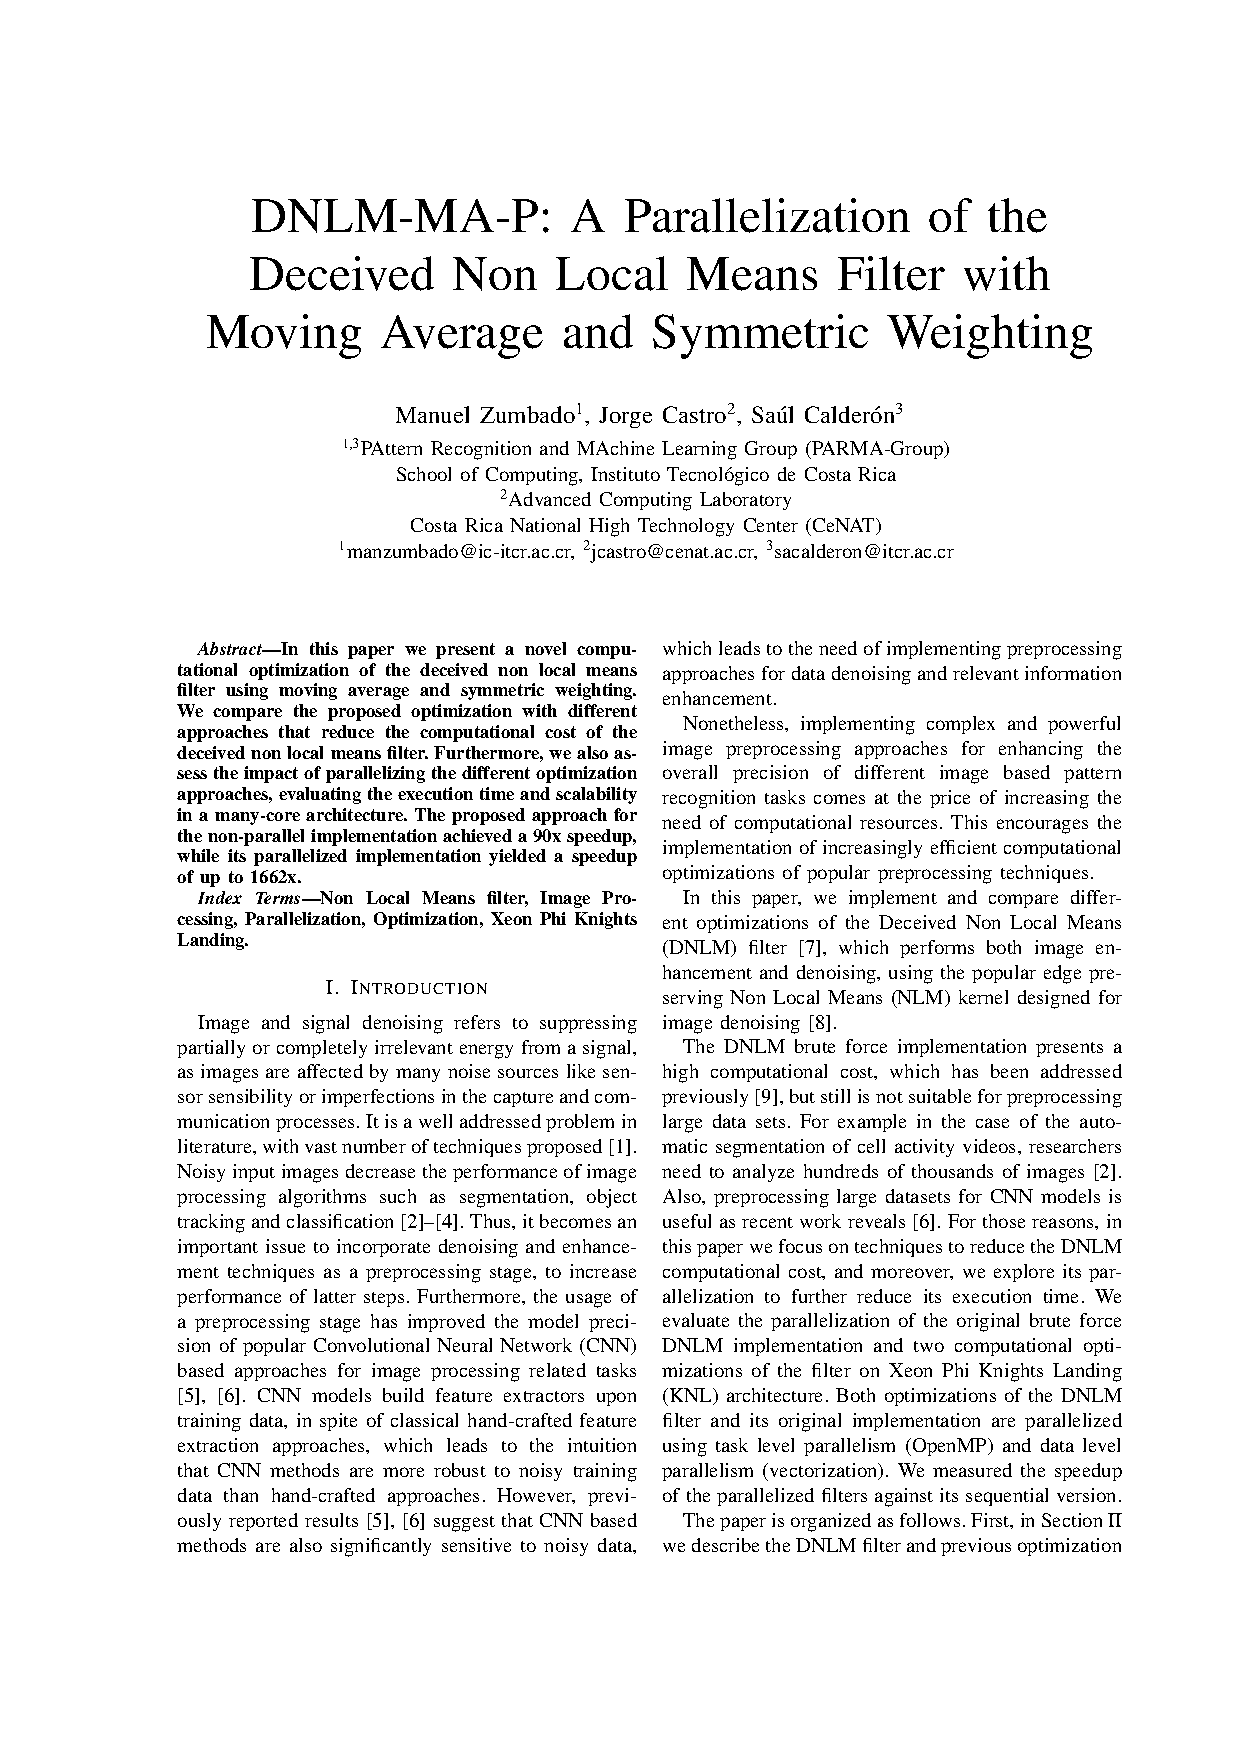
\includepdf[pages=-,pagecommand={},offset=75 -75]{papers/dnlm-ma-p}



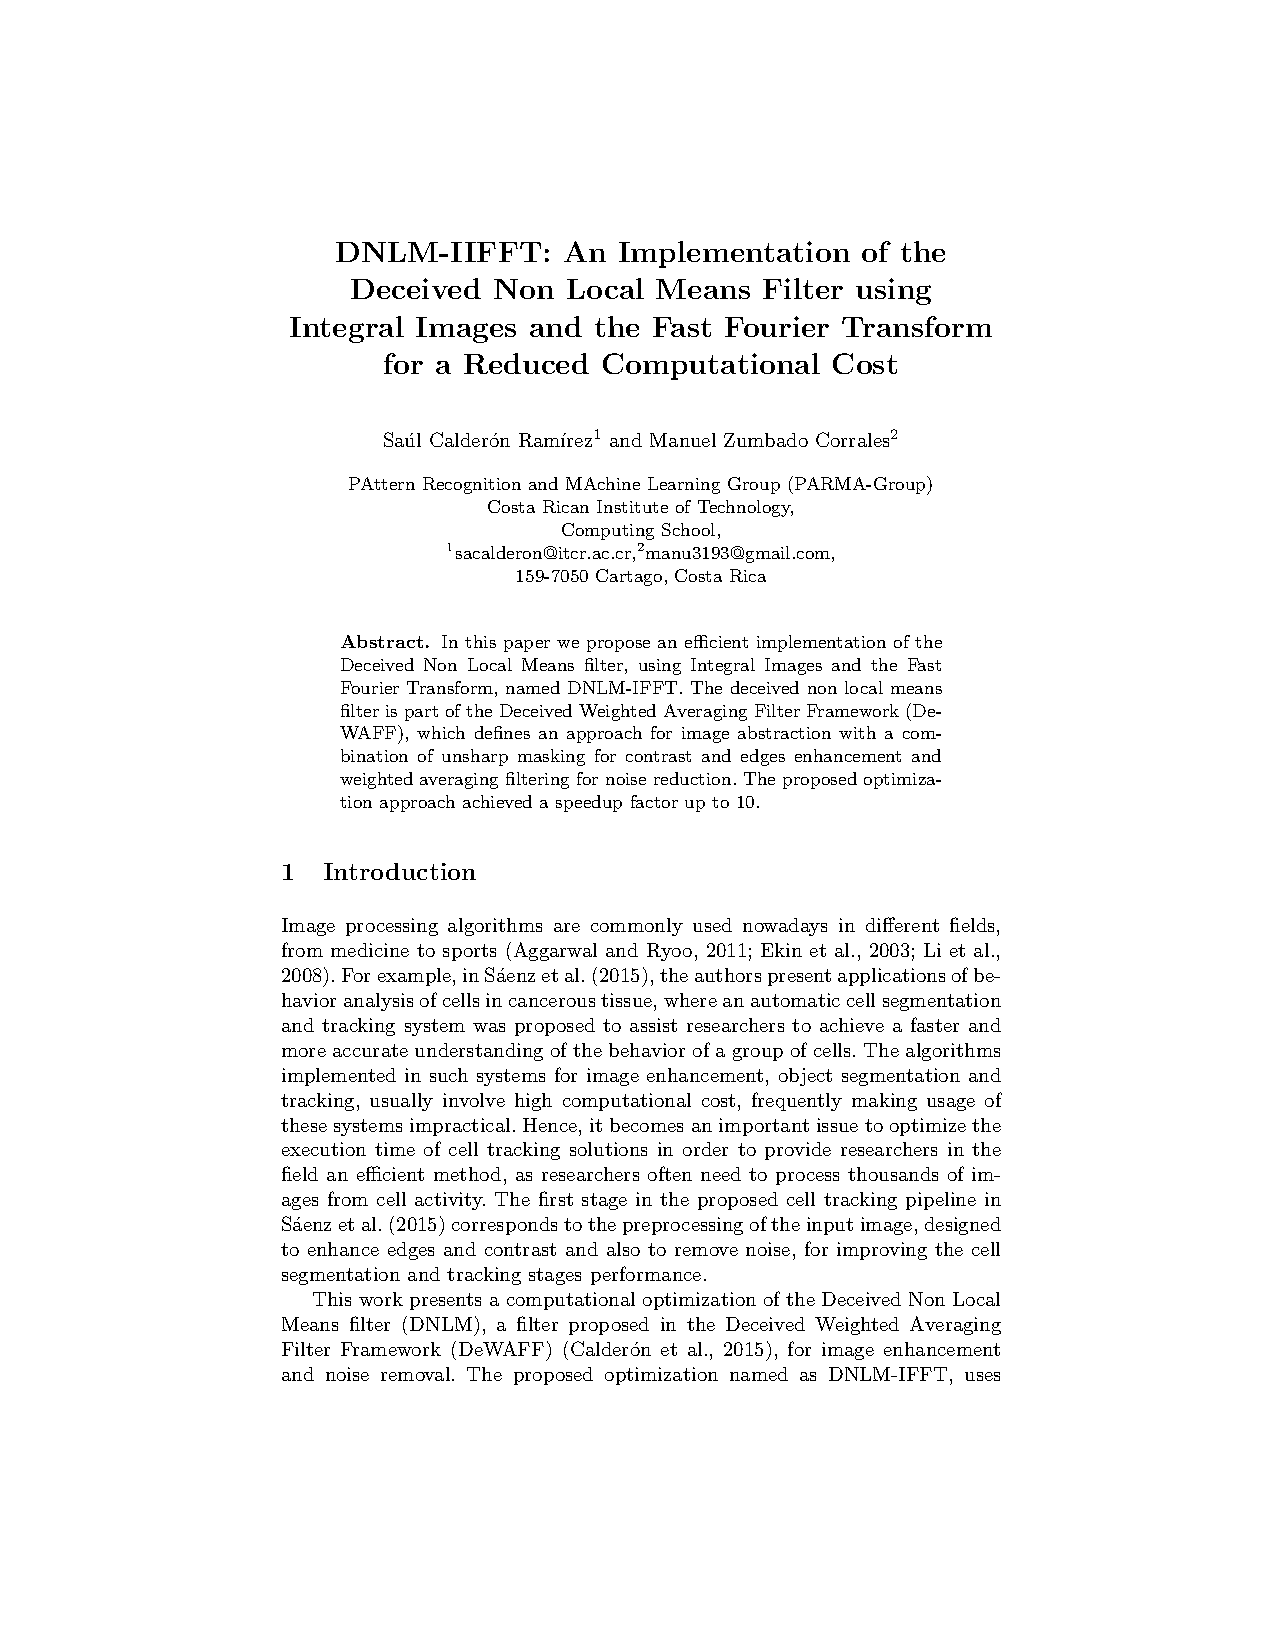
\includepdf[pages=-,pagecommand={},offset=75 -75]{papers/dnlm-iifft}


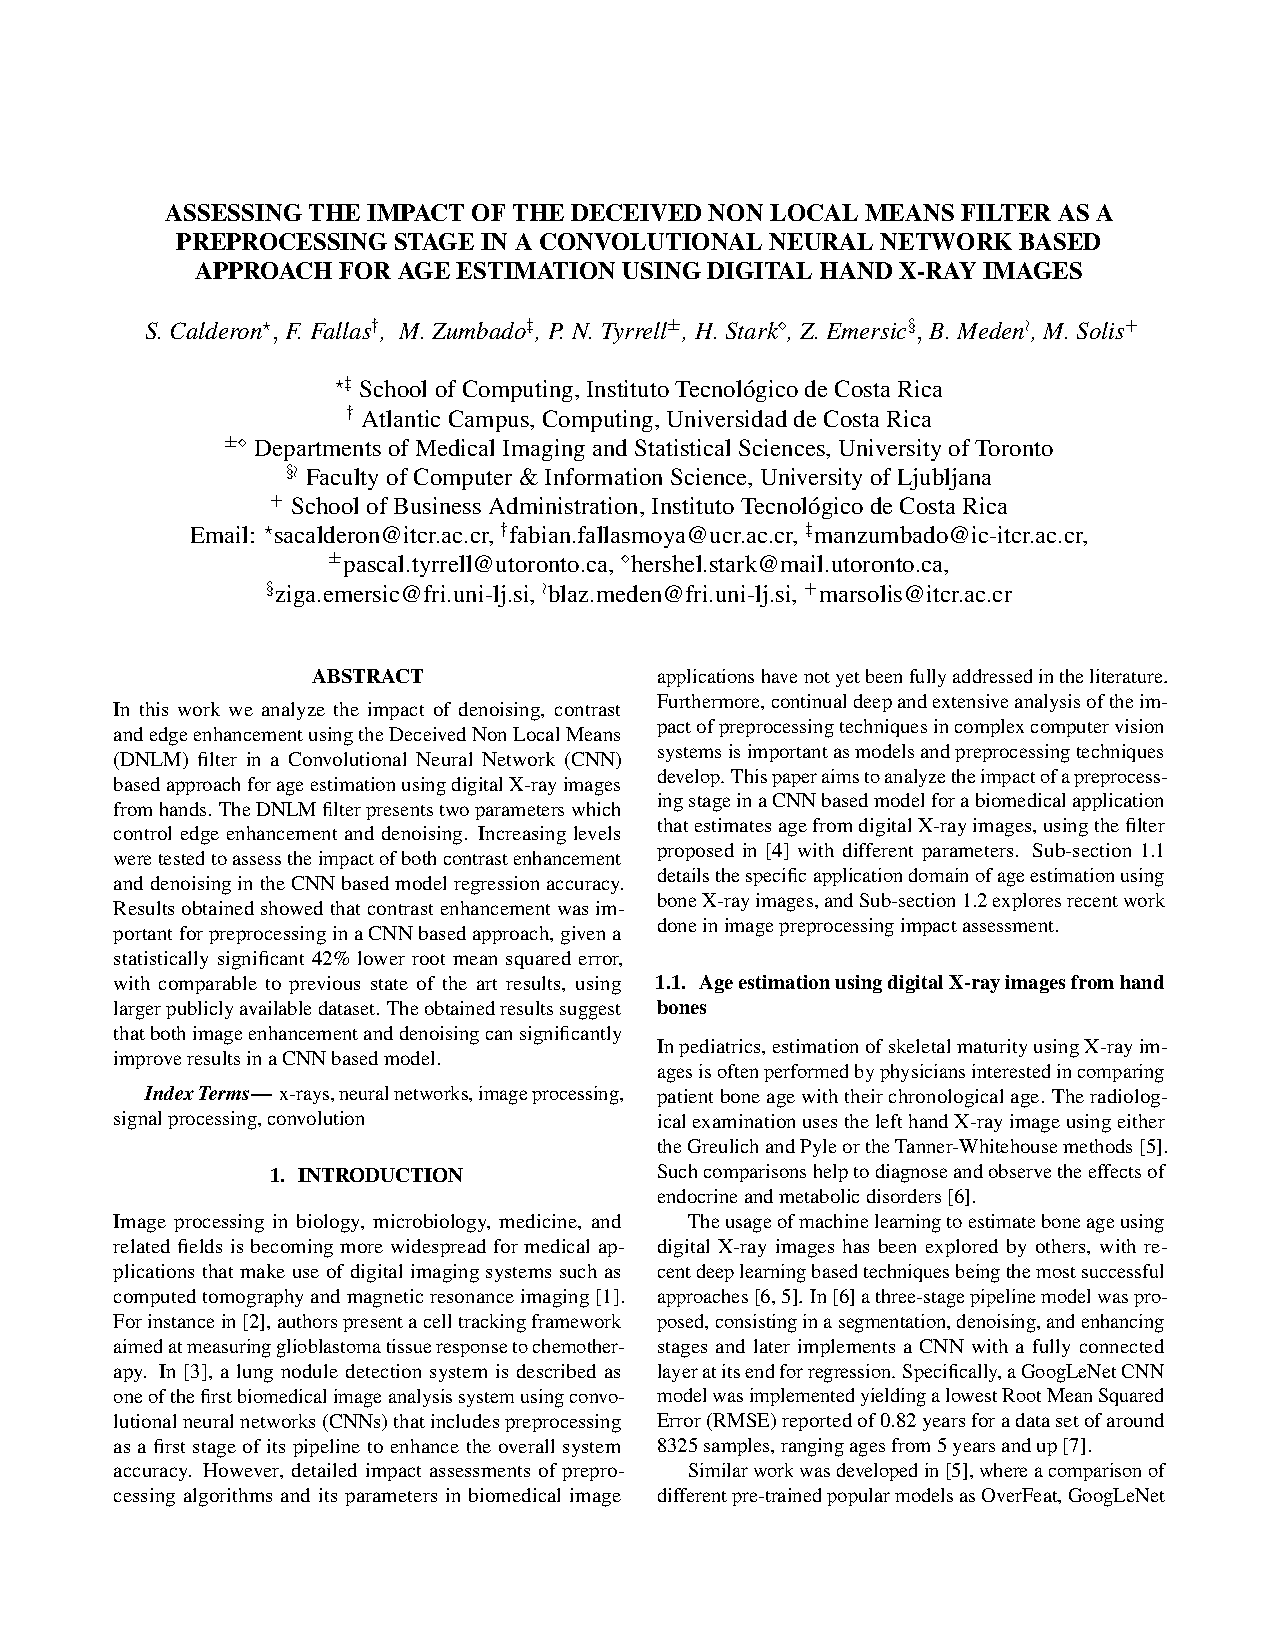
\includepdf[pages=-,pagecommand={},offset=75 -75]{papers/icip-2018}

  %----------------------------------------------------------------------------
  \backmatter
  %----------------------------------------------------------------------------

  \printindex                % insert index into document. Don't forget to call
                             % "makeindex filename" first.
\end{document}
